%! TEX rootmain.tex

\chapter{Jet-Switch Instruments}

Jet-switch instruments (flutes and flue organ pipes) share a common excitation principle: a thin air jet interacts with a sharp edge and an acoustic resonator. The chapter follows the physical chain from jet formation and instability, to jet-resonator coupling and the regenerative mechanism that sustains oscillation. Nonlinear effects, transients, mode transitions and aerodynamic noise are then introduced as natural consequences of the same feedback process, before closing with an overview of flute-type instrument families. 

\section{Dynamics of Air Jet}

\subsection{Jet Impingement on a Sharp Edge}

Even though the physical structure of these instruments varies a great deal, they all rely upon an air jet striking a sharp edge for excitation. The mechanics of a fluid jet entering an infinite body is a problem relevant in several application fields. Though conceptually simple, the underlying physics is complex and a first simplified treatment can be introduced by neglecting viscosity, compressibility and other non-idealities.

\paragraph{High-speed visualization} High-speed recordings of a jet striking a sharp edge show that the jet does not simply split into two steady streams. Instead, the impingement produces an unsteady roll-up of the shear layers and the formation of vortical structures close to the edge, so that the jet alternately feeds one side and then the other. This unsteady ``switching'' at the edge is the physical ingredient that later enables an oscillatory aeroacoustic source when the motion is synchronized with the resonator. This unsteady edge-switching is clearly visible in high-speed flow visualizations, as shown in figure \ref{fig:jet_edge_switching}.

\begin{figure}[!htb]
    \centering
    \subfloat{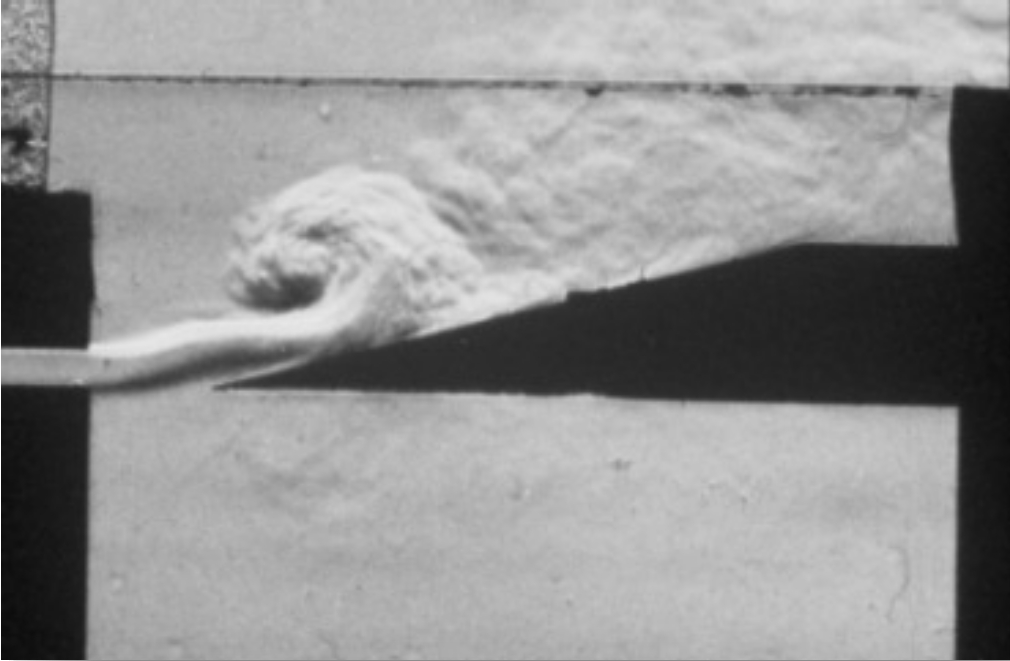
\includegraphics[width=0.3\linewidth]{00_Images/07_chapter/01_1.png}}\hfill
    \subfloat{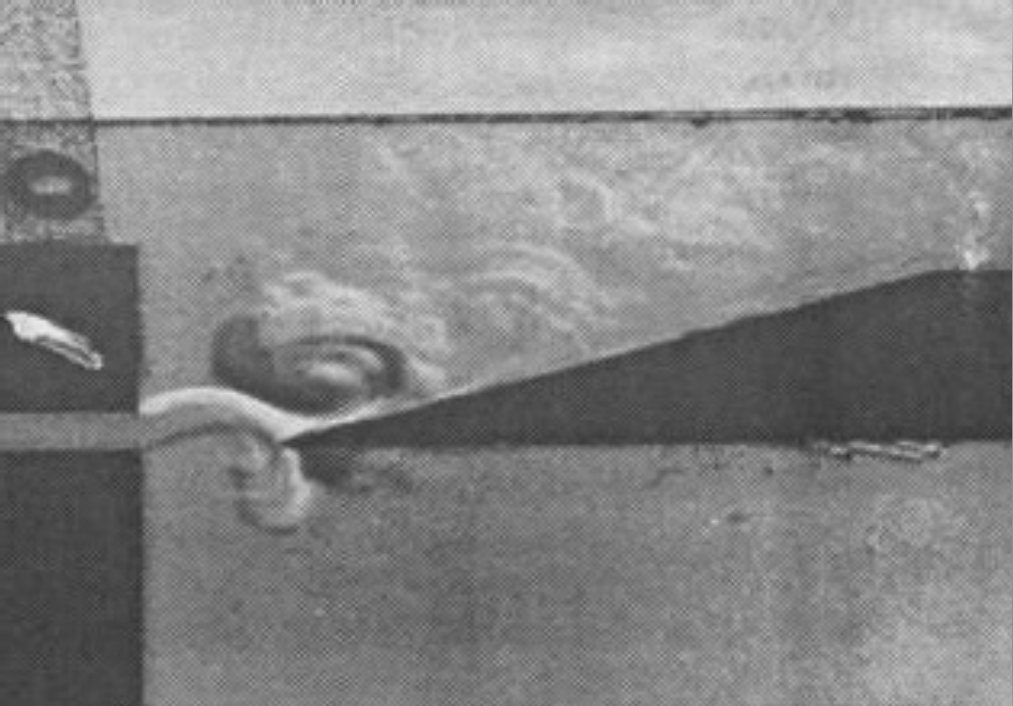
\includegraphics[width=0.3\linewidth]{00_Images/07_chapter/01_2.png}}\hfill
    \subfloat{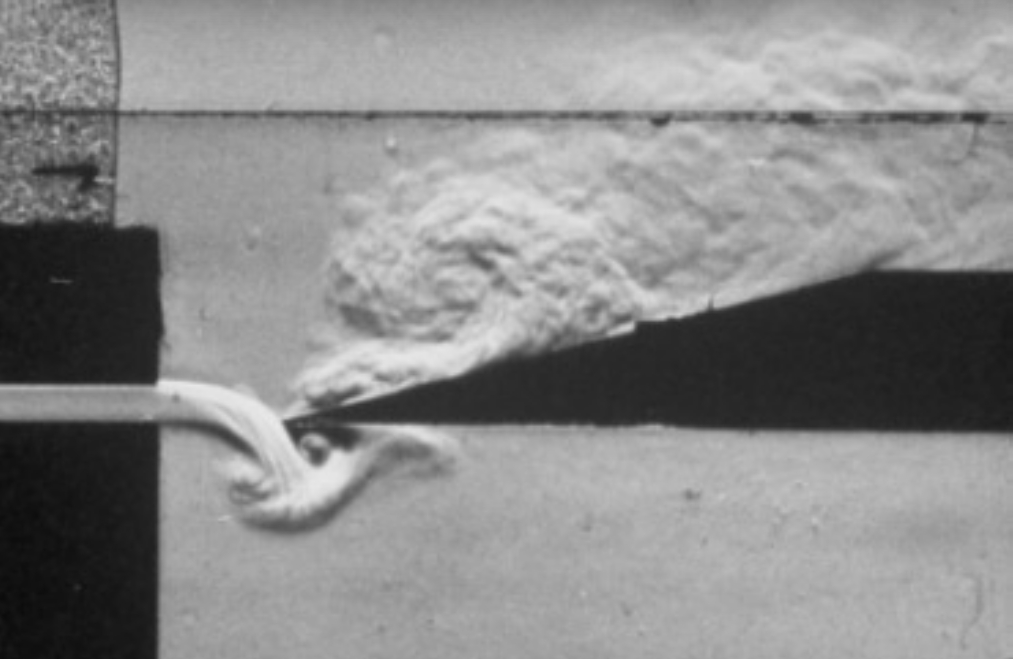
\includegraphics[width=0.3\linewidth]{00_Images/07_chapter/01_3.png}}
    \caption{High-speed visualization of jet switching at a sharp edge}
    \label{fig:jet_edge_switching}
\end{figure}

\subsection{Jet Instability and Convected Perturbations}

A qualitative analogy is provided by cigarette smoke. After a few centimeters, a thin smoke jet bends and oscillates and finally loses its organized structure, ending as a wide cloud. This kind of space-time instability can be observed as soon as two fluids with different velocities are in contact and it is greatly influenced by their relative velocity. In a flute, the air jet is blown across an open end of the pipe resonator. When jet oscillation occurs within the resonator, the jet instability can synchronize with the acoustic oscillation, resulting in a forced oscillation of the jet. The jet perturbation then grows as it is carried by the flow, being convected downstream toward the edge. 

\paragraph{Forced jet perturbation experiment} A clear illustration is obtained by forcing a transverse perturbation using loudspeakers placed a few centimeters apart from the flow, above and under it. In the reported setup the jet exhausts from the end of a \SI{1}{\milli\meter}-thick channel and the forced oscillation becomes visible as a growing waviness of the jet as it travels downstream. 

\subsection{Convection Velocity and Amplification}

Two characteristics of the jet motion are important for flue oscillation:

\begin{enumerate}
    \item the convection velocity of the perturbation, corresponding to the propagation velocity of the perturbation waves on the jet, which to a first approximation is about half the centerline jet velocity
    \item the amplification of the perturbation, corresponding to a characteristic growth factor of the instability waves along the jet
\end{enumerate}

Both characteristics depend on frequency, but the amplification depends strongly on it. The jet instability is stronger in a frequency range that depends on both jet velocity and jet thickness and the strongest amplification appears for frequencies around
\[
\frac{0.3U_j}{h}
\]
where \( U_j \) is the jet velocity and \( h \) is the thickness of the flue channel from which the jet is flowing. 

\section{Sound Generation}

Three main phenomena are involved in sound generation:

\begin{itemize}
    \item the perturbation of the jet by the acoustic field (jet receptivity)
    \item the evolution of the perturbation convected by the jet (jet instability)
    \item the production of acoustic energy by the perturbed flow (aeroacoustic sources)
\end{itemize}

The process can be summarized as a feedback loop: the pipe provides passive resonance and generates an acoustic field that perturbs the jet; the jet supports propagation and amplification of that perturbation while it is convected toward the edge; at the labium the perturbed jet acts as an aeroacoustic source that injects acoustic energy into the resonator, closing the loop. 

\section{Disturbance of an Air Jet}

\subsection{Terminology}

A reference terminology can be introduced using the recorder geometry. The air supply pressure is provided by the player’s mouth and drives a jet through the flue channel. The jet emerges at the flue exit and interacts with the labium, while the downstream pipe constitutes the resonator. The opening between the flue exit and the labium is called the mouth. Different names are adopted for organ pipes and transverse flutes, but the functional elements remain the same. The reference geometry and the associated naming conventions are summarized in figure \ref{fig:recorder_geometry_terms}.

\begin{figure}[!htb]
    \centering
    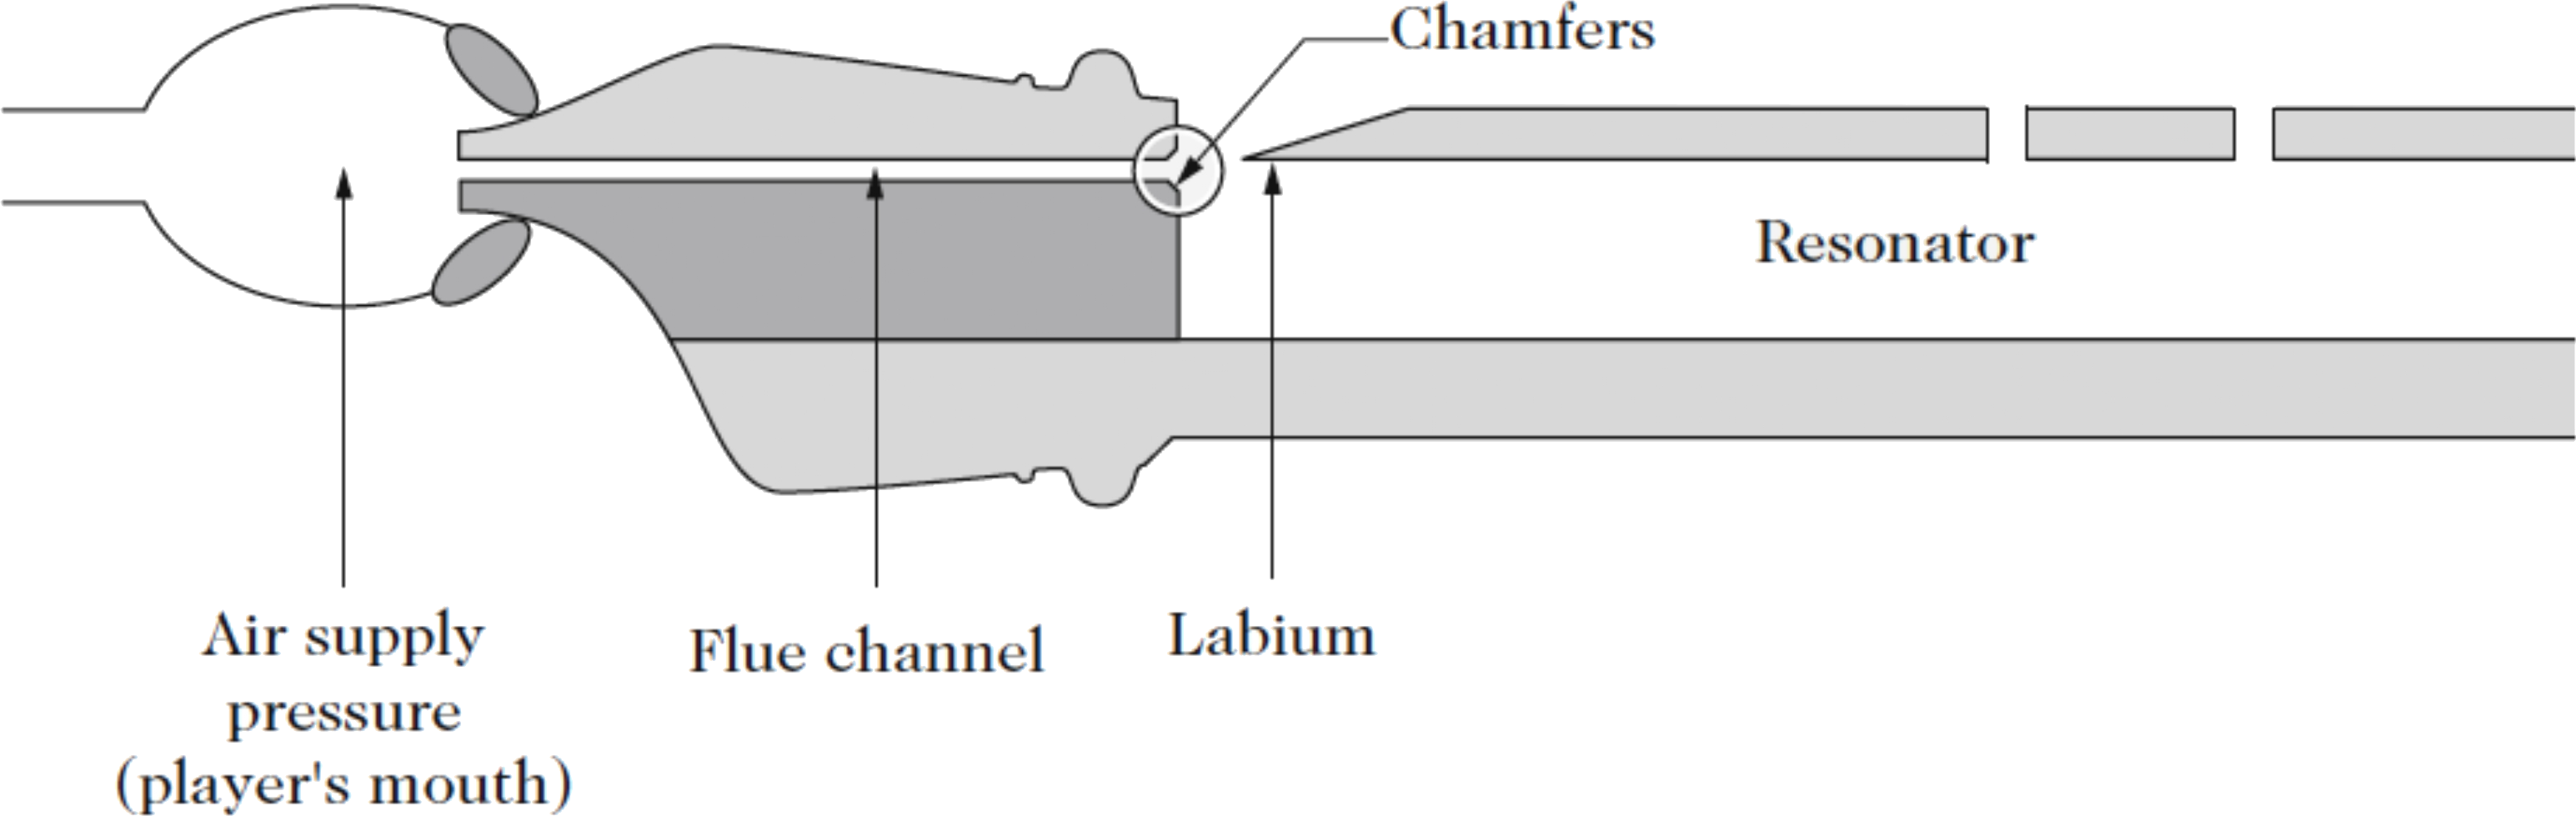
\includegraphics[width=0.7\linewidth]{00_Images/07_chapter/02.png}
    \caption{Recorder-like geometry and terminology for jet-switch instruments}
    \label{fig:recorder_geometry_terms}
\end{figure}

\subsection{Acoustic Sources at the Labium of the Flute}

The acoustic field at the flue exit induces a perturbation of the jet, which is amplified while being convected toward the labium. This process results in a transverse oscillation of the jet from one side of the labium to the other. A loop description makes the coupling more explicit. The acoustic field in the pipe resonator is responsible for the initial jet perturbation. The perturbation is then convected and amplified downstream due to the natural jet instability. The interaction of the perturbed jet with the labium constitutes the aeroacoustic source that feeds acoustic energy into the pipe. As a response to this excitation, the acoustic energy in the pipe is associated with an acoustic flow through the mouth, which in turn produces the jet perturbation at the flue exit, closing the feedback loop. 

\section{The Regenerative Excitation Mechanism}

\subsection{The Self-Sustained Oscillator as a Looped System}

The loop description allows predicting the oscillation frequency. Because the pipe accumulates energy only at resonances, the oscillation takes place at a frequency close to a passive pipe resonance. Stationary oscillations can occur when the total phase shift around the loop is \( 2\pi \) or any multiple of it. In a recorder gently blown, the time delay associated with the convection of perturbations is about half of the oscillation period, so the phase shift of the pipe must provide the complement to \( 2\pi \). For moderate blowing, the jet velocity increases and the convection delay decreases, so the delay associated with the pipe must increase. When blowing harder, the convection delay becomes too small compared to the period of the first pipe resonance and the oscillation jumps to the second pipe resonance, for which the same convection delay represents a larger phase shift. This regime jump is called overblowing. By blowing gently at very low pressures compared to standard playing, very soft tones can be produced at frequencies close to pipe resonances. This playing technique, called whistle-tones or sometimes eolian tones, corresponds to convection delays on the jet that are larger than one oscillation period. Values around one and a half or two and a half periods may be observed, instead of the half period typical of standard playing conditions. 

\subsection{Overblowing}

A simplified representation of the playing frequency of a flute as a function of jet velocity shows that oscillation occurs at a frequency close to one of the passive pipe resonances \( f_{1} \), \( f_{2} \), or \( f_{3} \). Regime changes do not occur at the same jet velocity when the jet velocity is increased versus decreased and a hysteresis appears. Dotted branches indicate whistle-tone oscillations. The typical evolution of the playing regime with jet velocity, including hysteresis and whistle-tone branches, is illustrated in figure \ref{fig:overblowing_hysteresis}.

\begin{figure}[!htb]
    \centering
    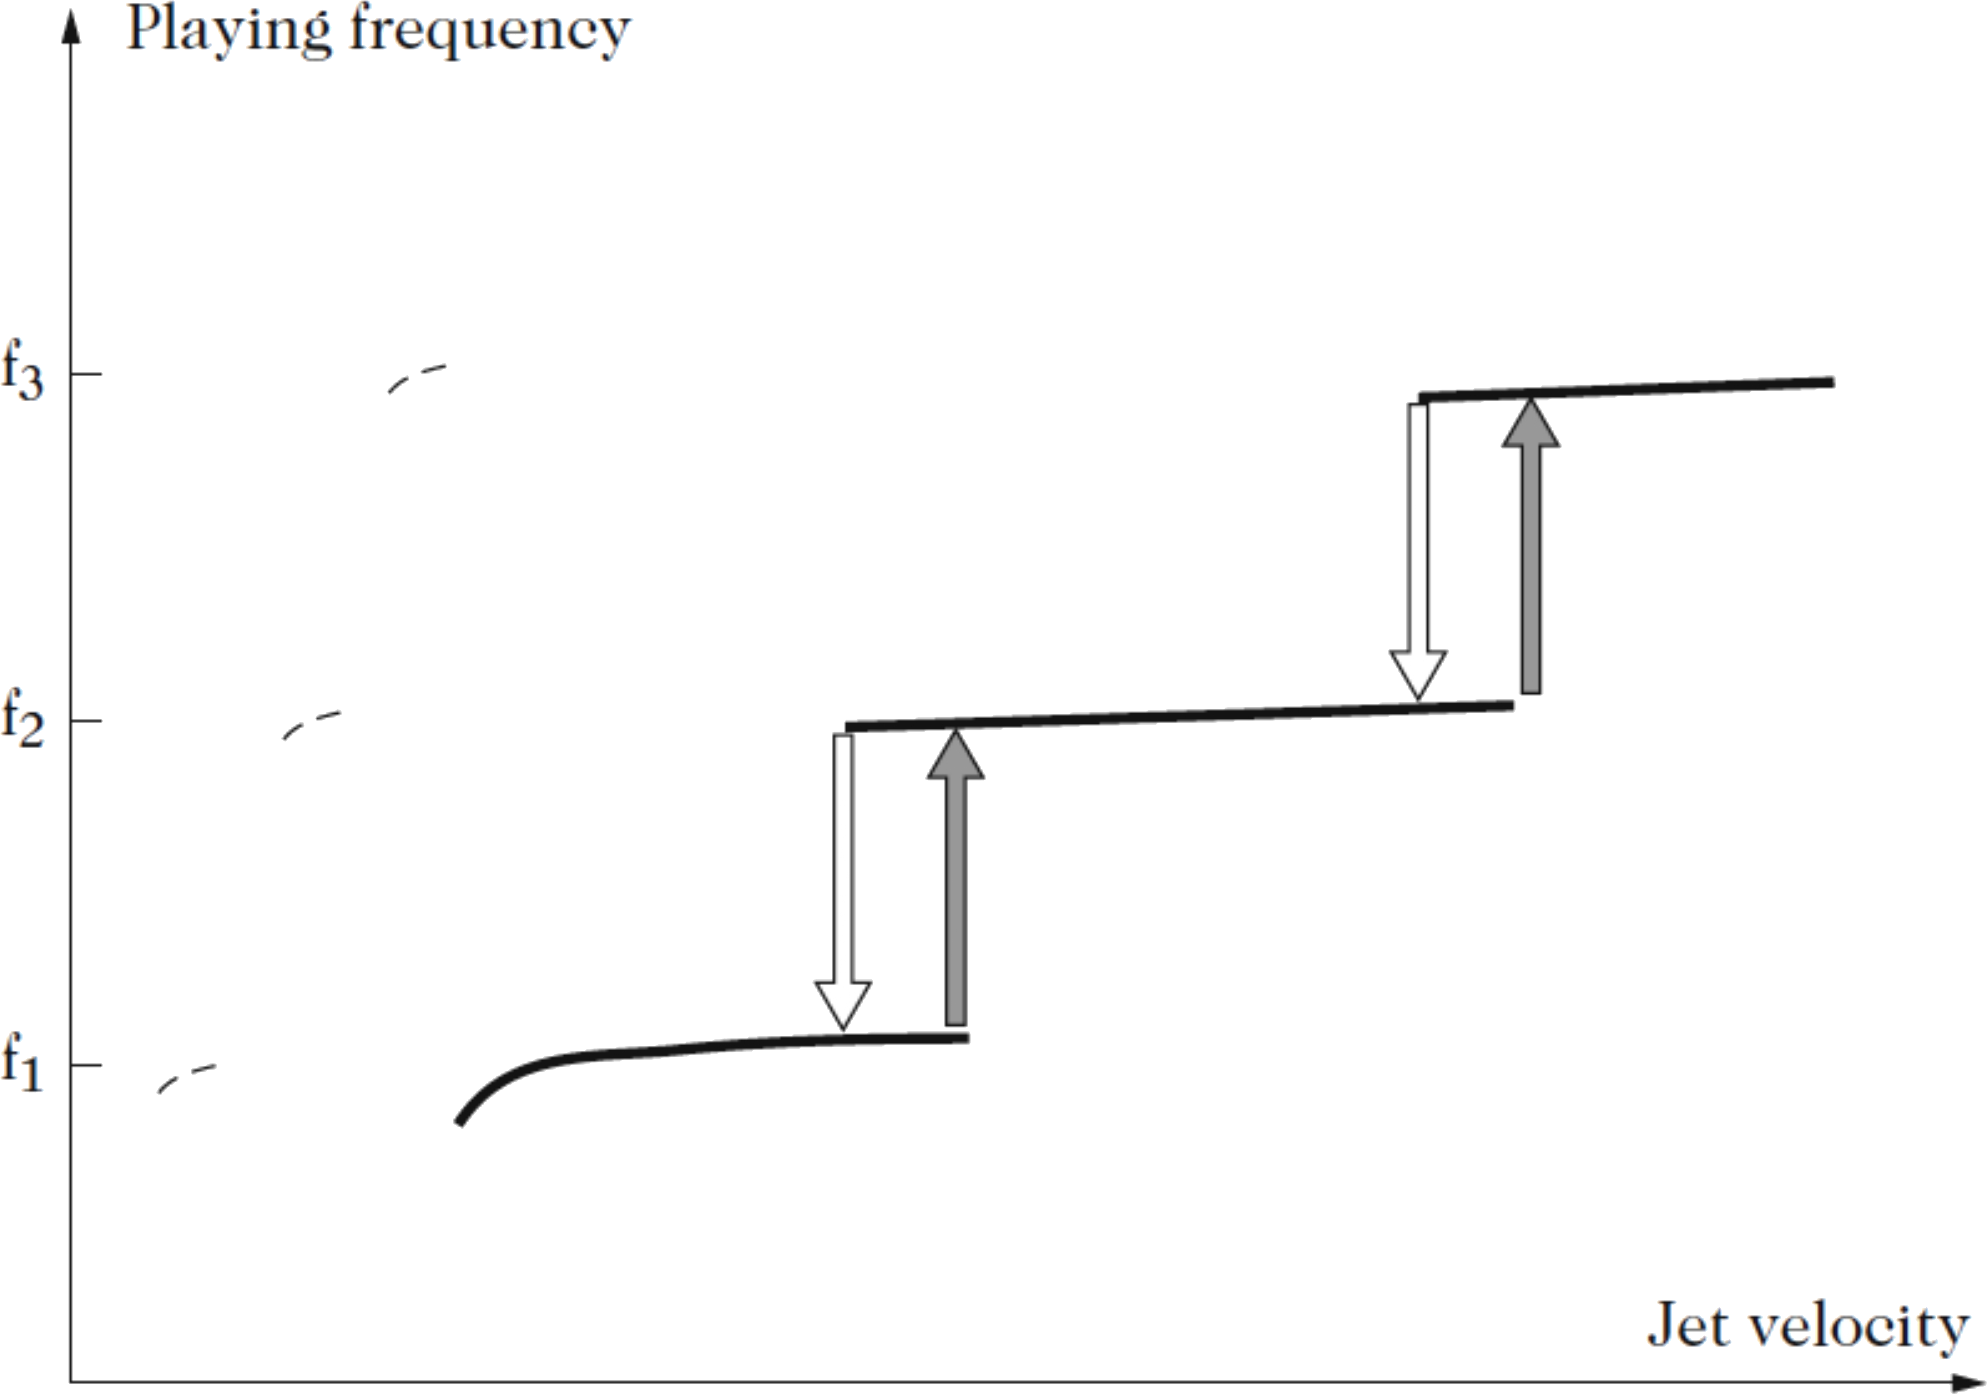
\includegraphics[width=0.7\linewidth]{00_Images/07_chapter/04.png}
    \caption{Overblowing and hysteresis of oscillation regimes versus jet velocity}
    \label{fig:overblowing_hysteresis}
\end{figure}

\section{The Sound of Flutes}

Using a mechanical air supply allows producing a stationary sound, as for an organ. The sound radiated by a pipe blown in this way can be split into two contributions: a deterministic part, analyzed in terms of sine-wave components and a stochastic part generated by turbulence. Turbulence produces broadband noise that is filtered by the pipe acoustical response. FFT analyses of internal pressure and radiated pressure measured at a distance of \SI{30}{\centi\meter} in front of the mouth of a small organ pipe illustrate this separation. At frequencies higher than the fifth harmonic, around \SI{2.5}{\kilo\hertz}, resonances can be identified through their filtering effect on the turbulence noise, because their frequencies do not coincide any more with the harmonic lines. The shift between harmonics and pipe resonances is visible, for example, when the sixth resonance lies between the harmonic lines 6 and 7. When the air supply comes from a player rather than from a mechanical system, pressure fluctuations modulate sound production. Vibrato corresponds to a conscious modulation of blowing, but fluctuations are also observed when the player aims at producing a stable tone. Because of these fluctuations, it is generally not possible to define a stationary part of the tone. Starting transients are also difficult to analyze: the sound components that later become the harmonics of the steady part display changing frequencies and amplitudes during the attack transient. In the reported example of the time evolution of the first three frequency components, the second component, with frequency close to twice that of the later fundamental, increases much faster than the first component. The deterministic harmonic lines and the turbulence-driven broadband component can be distinguished in measured spectra, as shown in figure \ref{fig:pipe_fft_deterministic_stochastic}, where a time evolution of the first three frequency components during an attack transient is also reported.

\begin{figure}[!htb]
    \centering
    \subfloat[Spectra]{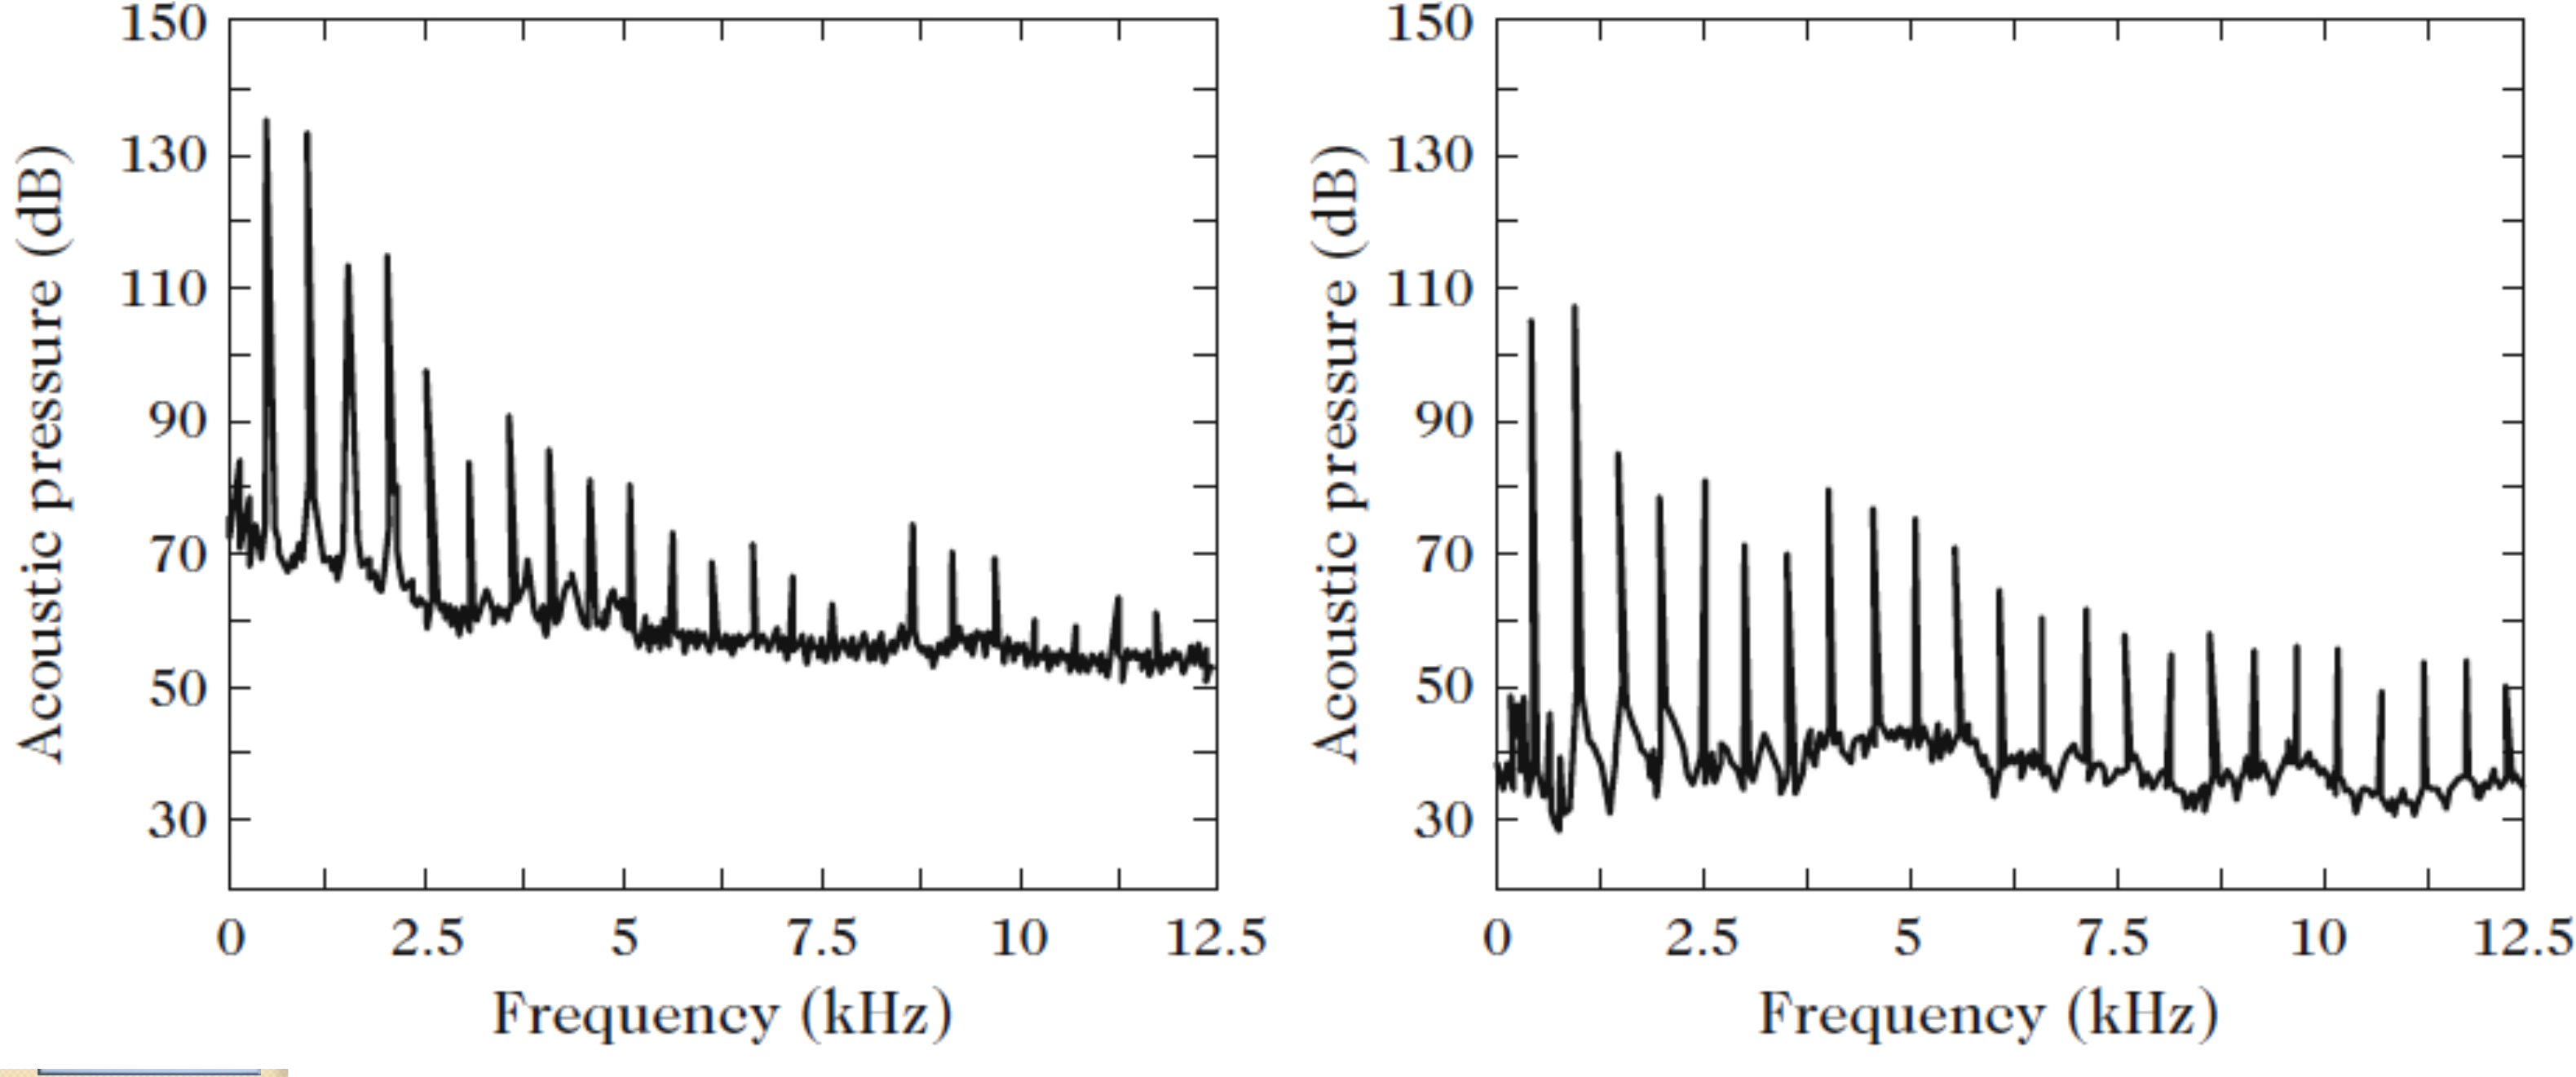
\includegraphics[height=0.17\textheight]{00_Images/07_chapter/05.png}}
    \subfloat[Time evolution]{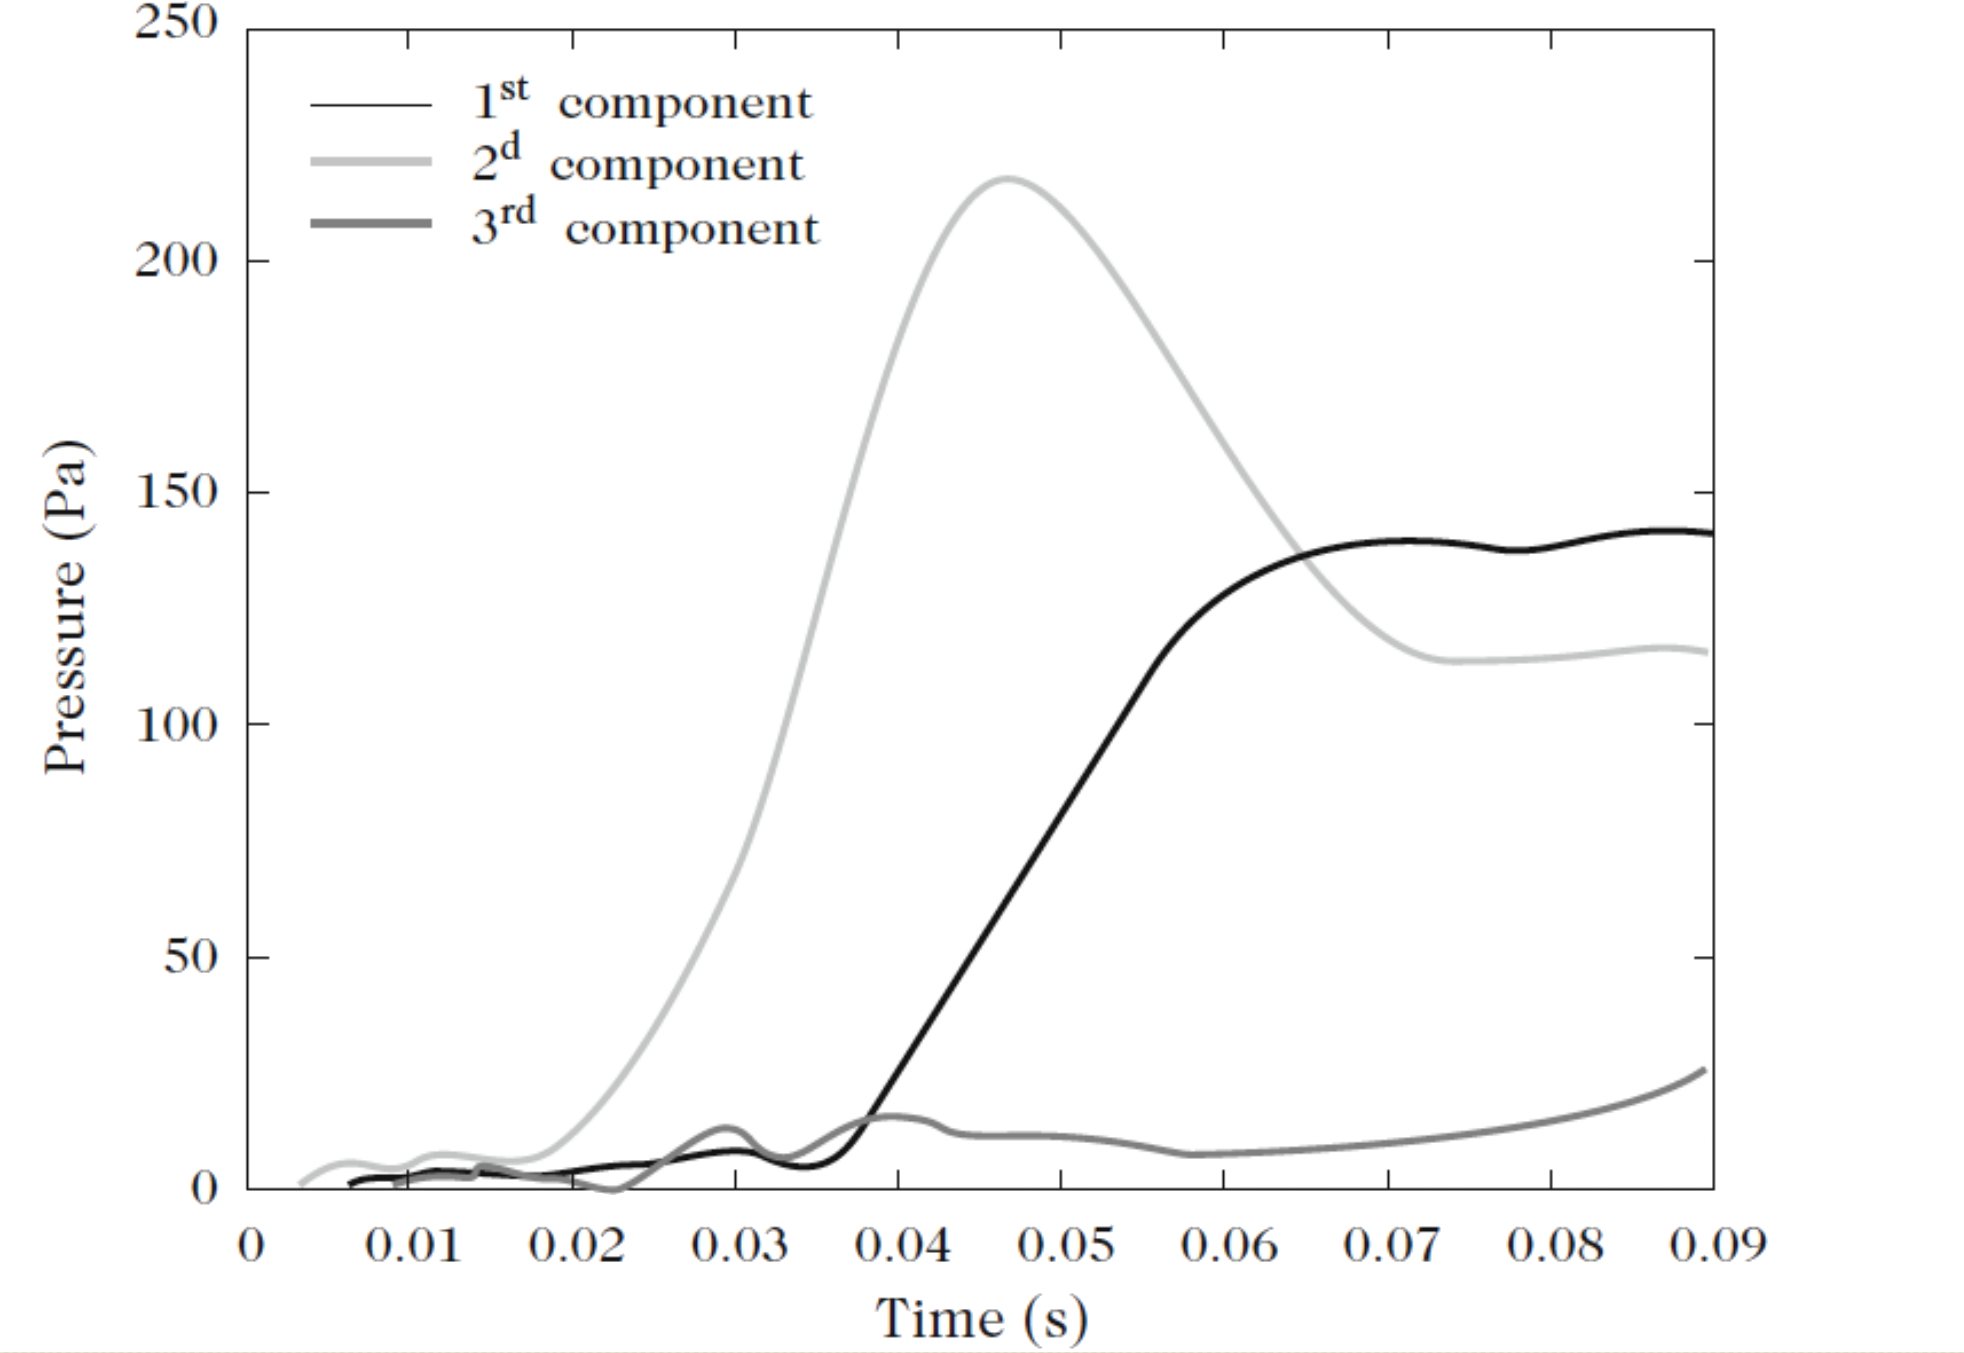
\includegraphics[height=0.17\textheight]{00_Images/07_chapter/06.png}}
    \caption{Measured spectra and time evolution showing harmonic components and turbulence noise filtered by resonances}
    \label{fig:pipe_fft_deterministic_stochastic}
\end{figure}

\section{Jet-Resonator Interaction}

\subsection{A Global Model of the Instrument}

A global model is most straightforward for jet-driven instruments whose geometry remains essentially fixed during playing, such as flue organ pipes and recorders. In this case, the excitation system can be described by a small set of stable parameters (channel geometry, jet velocity, flue exit--labium distance) coupled to the passive acoustic response of the resonator. Transverse flutes are more complex because the jet is shaped by the player’s lips, so the effective geometry and jet parameters can vary continuously during performance and become part of the control strategy. 

\subsection{Parameters of the Model}

\begin{figure}[!htb]
    \centering
    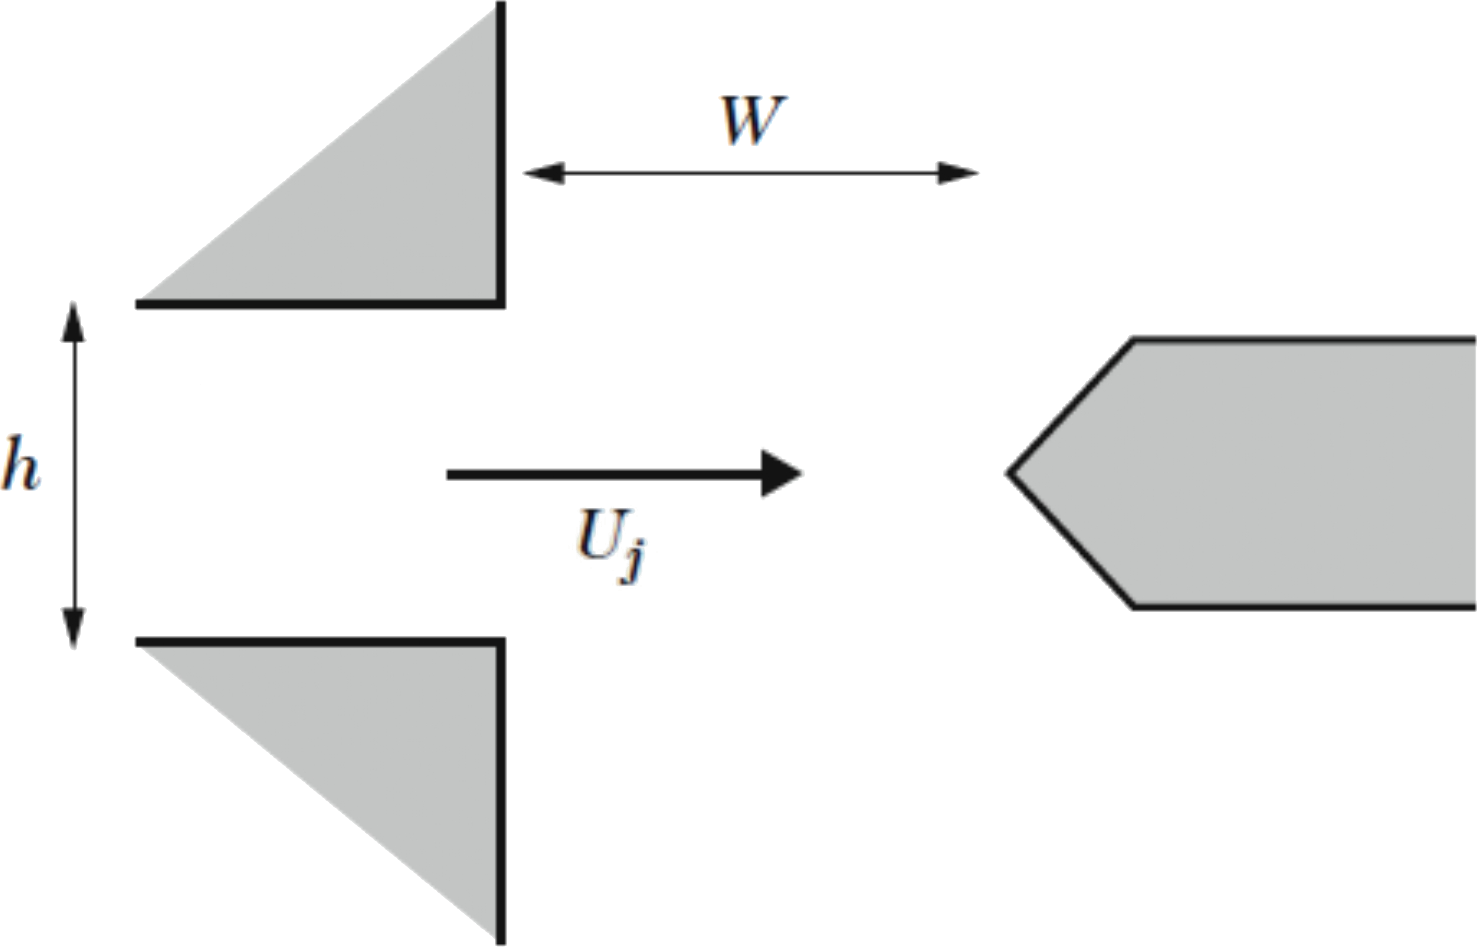
\includegraphics[width=0.5\linewidth]{00_Images/07_chapter/07.png}
    \caption{Simplified geometry}
    \label{fig:geom}
\end{figure}

A minimal geometric (reported in figure \ref{fig:geom}) and flow description introduces the channel thickness \( h \), the central jet velocity at the channel exit \( U_j \) and the flue exit--labium distance \( W \). The transverse jet displacement can be decomposed as
\[
y(x,t) = y_{0}(x,t) + y_{\mathrm{ac}}(x,t)
\]
and the corresponding transverse velocity as
\[
v(x,t) = v_{0}(x,t) + v_{\mathrm{ac}}(x,t)
\]
The jet regime is characterized by the Reynolds number
\[
\Re\{y\} = \frac{U_j h}{\nu}
\]
where \( \nu \) is the kinematic viscosity. Typical values range from a few hundreds (recorder) up to about \( 10^{4} \) in modern transverse flute playing, with
\[
500 < \Re\{y\} < 10000
\qquad
\nu = \SI{1.5e-5}{\meter\squared\per\second}
\]
Jet instability is characterized by a Strouhal number (inverse dimensionless frequency). Two common definitions are
\[
\frac{\omega W}{U_j}
\qquad
\frac{fh}{U_j}
\]
For normally blown flutes, one half hydrodynamic wavelength is observed between flue exit and labium, leading to
\[
\mathrm{St}_{W} = \frac{fW}{U_j} \approx 0.25
\]
A convenient measure of oscillation level is the ratio between the acoustic perturbation velocity in the mouth and the central jet velocity, typically
\[
\frac{V_{\mathrm{ac}}}{U_j} \approx 10^{-1}
\]

\subsection{The Flow in the Channel}

Knowing the overpressure \( \Delta p \) in the reservoir (player’s mouth) with respect to atmospheric pressure leads to an estimate of the central jet velocity,
\[
U_j = \sqrt{\frac{2\Delta p}{\rho_0}}
\]
The Bernoulli estimate holds at the center of the flow. Near the walls, viscosity produces boundary layers whose thickness at position \( x \) along the channel is approximated by
\[
\delta(x) \approx \sqrt{\frac{\nu x}{U}}
\]
In a short channel, boundary layers remain confined near the walls and the central part of the flow exhibits an approximately uniform velocity profile. In a long channel, the two boundary layers merge and a parabolic (Poiseuille) profile develops. In most flutes, the Bernoulli approximation (uniform velocity) is a reasonable working model. 

\subsection{The Jet Flowing out of the Channel}

At the channel inlet, the flow has an approximate top-hat velocity profile. As the fluid flows downstream, boundary layers thicken because of viscosity. If the channel outlet is rounded, the flow slows down, producing an increase of pressure. The change of sign of the pressure gradient in the diverging part at the channel exit is responsible for flow separation. Because of viscosity, the free jet entrains the surrounding fluid. This behavior is reported in figure \ref{fig:jetflowing}.

\begin{figure}[!htb]
    \centering
    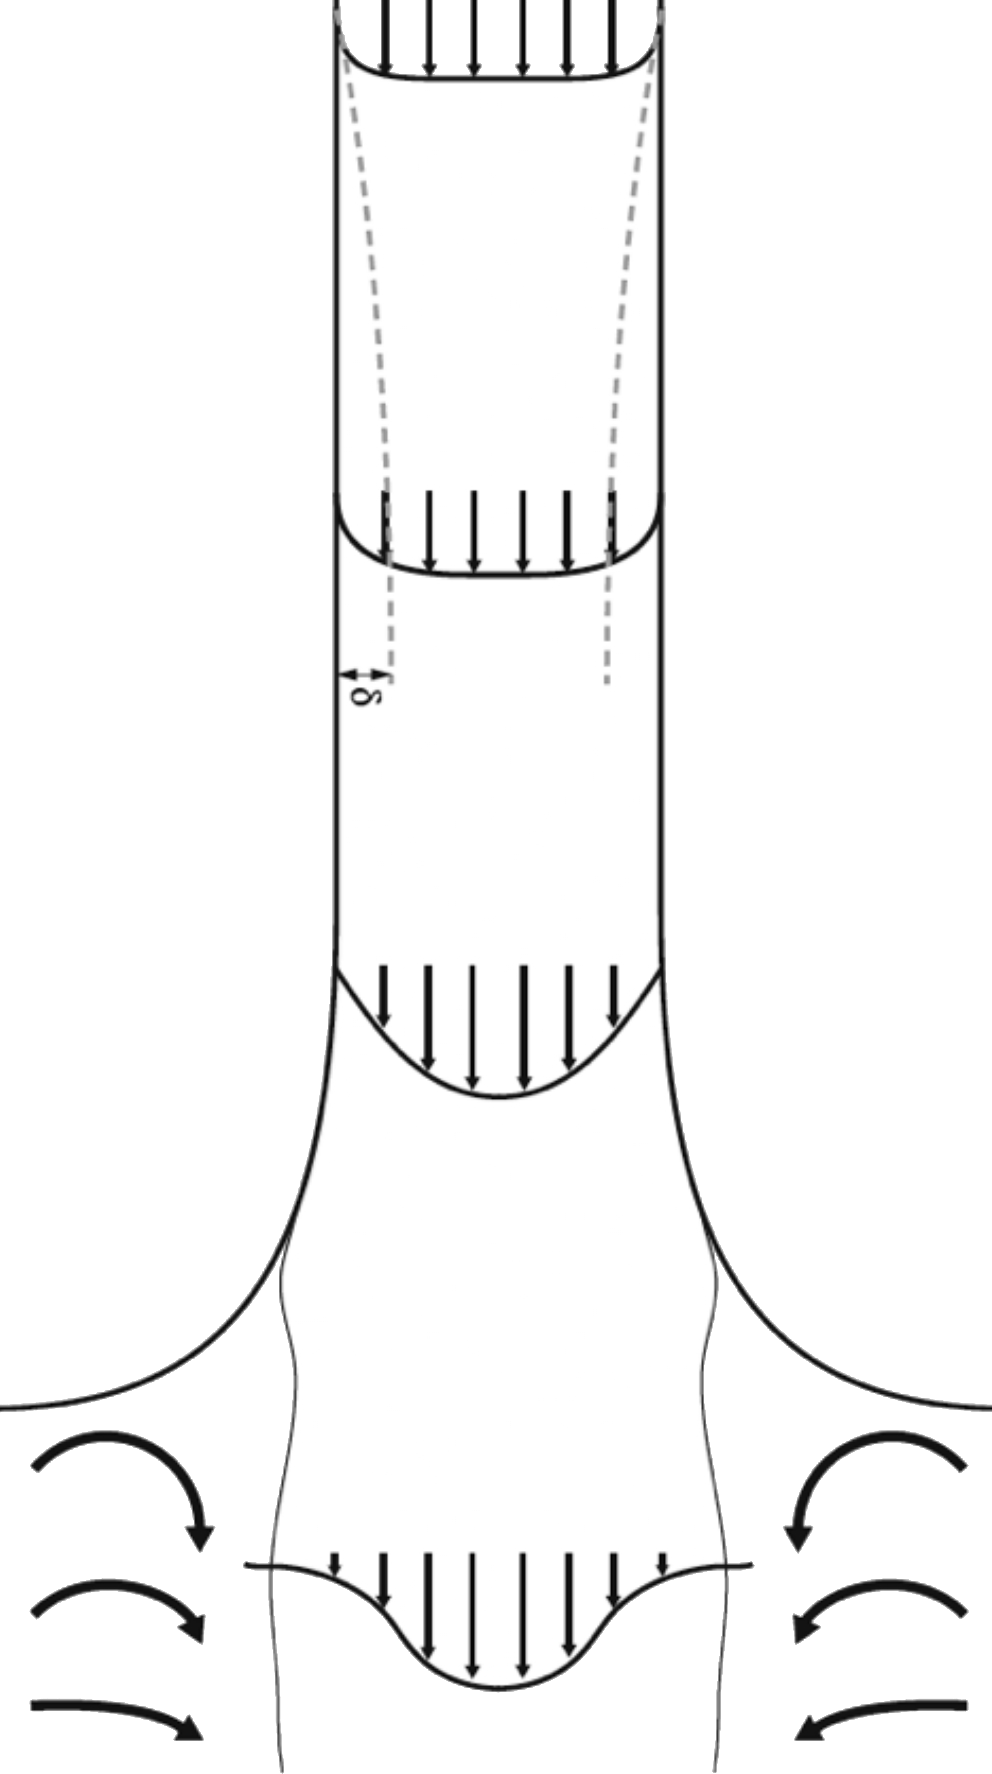
\includegraphics[height=0.7\linewidth,angle=90]{00_Images/07_chapter/10.png}
    \caption{Jet flowing out of the channel}
    \label{fig:jetflowing}
\end{figure}

\section{Jet Instability}

\subsection{Assumptions}

A first physical description of jet instability is introduced under the following assumptions:

\begin{itemize}
    \item inviscid fluid
    \item compressibility can be ignored, which is justified
    \begin{itemize}
        \item as long as the jet velocity \(U\) is kept small compared to the sound speed \(c\)
        \item as long as the dimensions of the jet and sound production region are small compared to the acoustic wavelength
    \end{itemize}
\end{itemize}

\subsection{Kelvin-Helmholtz Instability}

Let us start the physical analysis of the jet instability with a simple case: the flow at the planar interface between two areas of the fluid with different velocities. This is known as the Kelvin-Helmholtz instability. This flow can be described by the relative velocity \(U\) between the two areas,
\[
v_x = \frac{U}{2} \quad \text{if } y>0
\qquad
v_x = -\frac{U}{2} \quad \text{if } y<0
\qquad
v_y = 0
\]

\subsection{The Instability Mechanism}

The instability mechanism of a perturbed shear layer can be summarized as follows (and visualized in figure \ref{fig:instmech}):
\begin{itemize}
\item a perturbation of the interface induces local convection that concentrates the vorticity at points \(C\)
\item this concentration amplifies the initial perturbation, leading to the formation of rolled structures
\item vorticity accumulation induces asymmetrical velocities that further amplify the initial perturbation, up to the point where waves break
\end{itemize}

\begin{figure}[!htb]
    \centering
    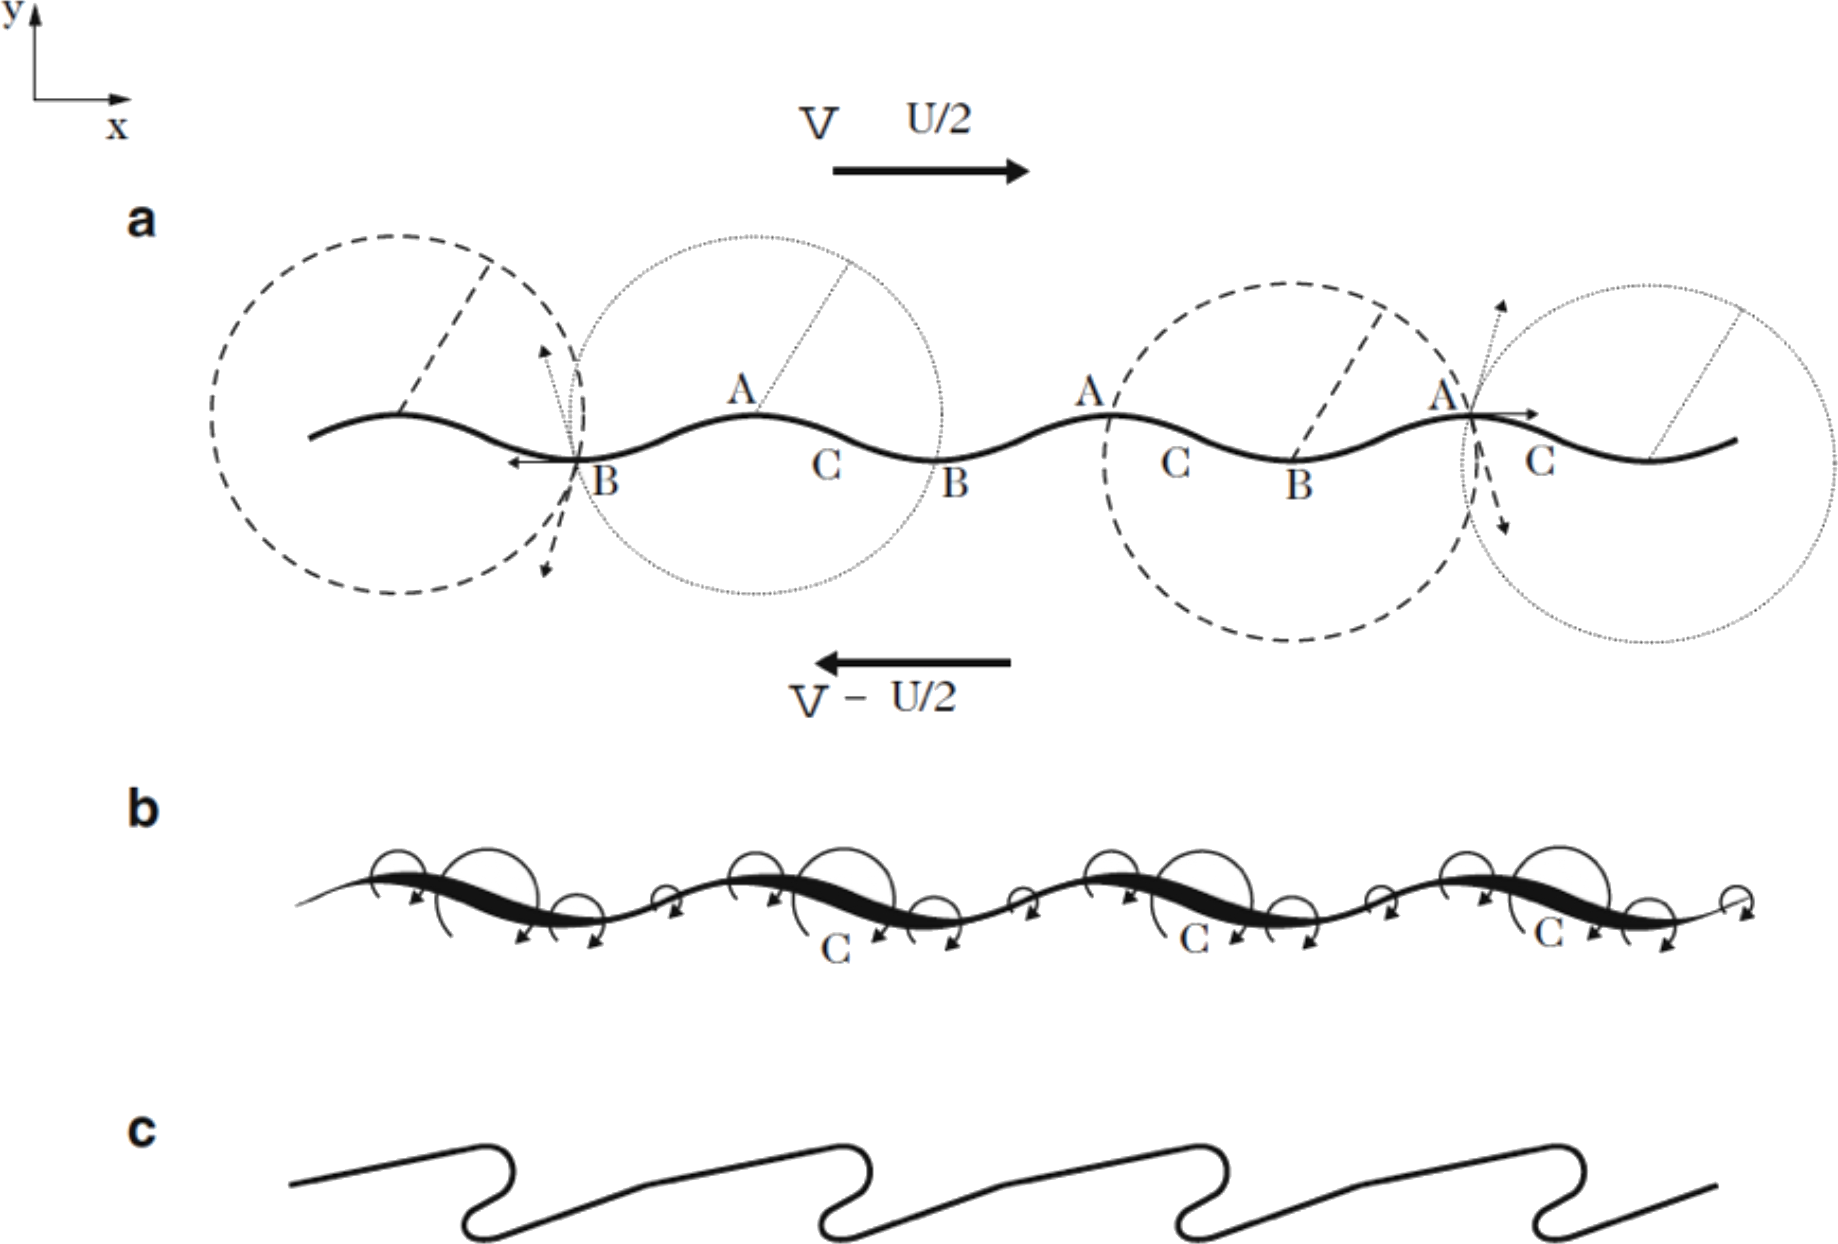
\includegraphics[width=0.7\linewidth]{00_Images/07_chapter/11.png}
    \caption{Instability mechanism}
    \label{fig:instmech}
\end{figure}

\subsection{Instability of an Infinite Jet}

If the jet velocity profile is symmetrical about \(y=0\), perturbations on both shear layers of the jet can be symmetrical or anti-symmetrical, depending on the symmetry properties of the initial perturbation of the jet.

\begin{itemize}
    \item Symmetrical perturbations induce the so-called varicose oscillations of the jet, associated with a modulation of the jet thickness.
    \item Anti-symmetrical perturbations correspond to sinuous oscillations of the jet. Sinuous oscillations have a stronger amplification than varicose oscillations.
\end{itemize}

Jet visualizations in various flute configurations indicate that the sinuous motion dominates under standard blowing conditions. The distinction between varicose and sinuous oscillations is summarized by the mode sketches in figure \ref{fig:varicose_sinuous_modes}.

\begin{figure}[!htb]
    \centering
    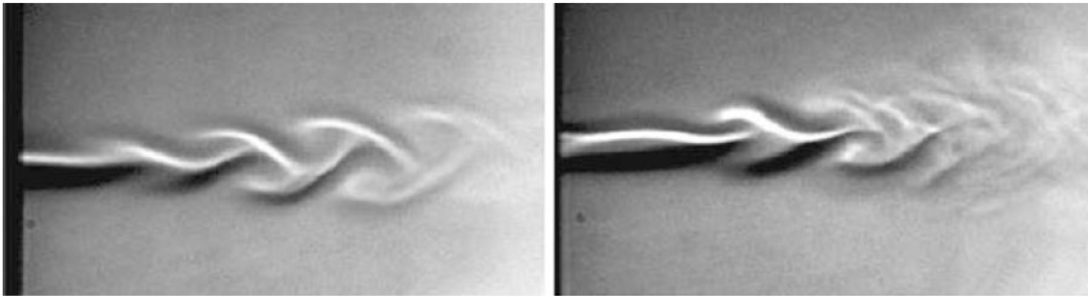
\includegraphics[width=0.7\linewidth]{00_Images/07_chapter/12.png}
    \caption{Varicose and sinuous jet oscillation modes}
    \label{fig:varicose_sinuous_modes}
\end{figure}

\subsection{Spatial Amplification}

It is of interest the study of the spatial amplification of the instability. Introducing a complex wavenumber,
\[
\alpha = \alpha_r + j\alpha_i
\]
the amplitude of the oscillation is proportional to
\[
e^{\alpha_i x}
\]
where \( \alpha_i \) is the spatial growth rate and \( \alpha_r \) controls the space periodicity. The amplification depends on the jet velocity profile and corresponds to anti-symmetrical jet oscillations (sinuous) or symmetrical oscillations (varicose), with sinuous oscillations being better amplified than varicose oscillations.

\section{Jet Receptivity}

\subsection{Localization of the Initial Perturbation}

The way the acoustic field produces the initial jet perturbation is called the receptivity. To a first approximation, the initial perturbation is assumed to be localized at the flue exit. In an incompressible inviscid flow approximation, this can be justified by vorticity conservation in the flow. The jet perturbation can be represented as a modulation of vorticity in the flow. Because of vorticity conservation, such a vorticity modulation can only be injected at the separation points of the flow, due to local viscous effects. The amplification that occurs downstream is only a consequence of the jet instability, in terms of redistribution of the initial vorticity.

\subsection{Influence of Geometry}

Details of the geometry and of the flow in the vicinity of the flow separation points can strongly affect the receptivity:

\begin{itemize}
    \item boundary layer thickness in the channel just upstream from the flue exit
    \item geometry of the channel exit
\end{itemize}

This is in line with recorder makers’ care in cutting chamfers at the end of the channel and with transverse flute players’ observation that small irregularities on the lips strongly affect tone quality.

\subsection{Semi-Infinite Jet Model}

The theory behind varicose and sinuous motions is valid for an infinite parallel flow. In flutes, the jet is formed at the flue exit and flows through a window where strong transverse acoustic flows can be experienced, due to the accumulation of acoustical energy in the pipe resonator. A first step is to consider a semi-infinite jet with negligible transverse displacement at the flue exit. The transverse displacement \( \eta(x,t) \) of the jet in the \(y\) direction can be calculated by integration of the transverse velocity from the flue exit to the current position \(x\) in the mouth. This transverse velocity is made of two components: a perturbation term \(v'_y\) exponentially growing with the distance from the flue exit and the air displacement due to the acoustic velocity \(v_{\mathrm{ac}}\),
\[
\eta(x,t)=\int_{t-x/U_0}^{t}\Bigl[v'_y(x',t')+v_{\mathrm{ac}}(x',t')\Bigr]dt'
\qquad
x' = x - (t-t')U_0
\]

\subsection{Exponential Growth}

For long enough distances from the flue exit, one can ignore the contribution of the acoustic displacement. The transverse jet displacement then writes
\[
\eta(x,t)\approx -\int_{t-x/U_0}^{t}\frac{\partial\psi'(x',t')}{\partial x}dt'
\]
where \( \psi' \) is the perturbation amplification function. This implies an exponential growth of the amplitude of the jet displacement.

\subsection{Experimental Model of Receptivity}

A good experimental model of the receptivity is given by
\[
\eta(x,t)\approx \eta_0e^{\alpha_i x}e^{j\omega\left(t-x/c_p\right)}
\qquad
x>h
\]
with
\[
\eta_0=\frac{V_{\mathrm{ac}}h\delta_j}{U_j\delta_{\mathrm{ac}}}
\qquad
\delta_j=\frac{L}{\sqrt{\Re\{y\}}}
\qquad
\delta_{\mathrm{ac}}=\sqrt{\frac{2\nu}{\omega}}
\]
where \(c_p\) is the velocity of convection of the perturbation and \(L\) is the flue channel length.

\section{Jet Roll Up and Vortex Formation}

For jet transversal displacement of the same order of magnitude as the jet thickness, the jet appears to roll up and break down into discrete vortices. The flow can then be described as an alternate vortex street, as described by Von K\'arm\'an. In order to be stable, the vortex street needs to follow the correct relation between the hydrodynamic wavelength \( \lambda_h \), the street width \( b \), the circulation \( \Gamma \) of vortices and the convection velocity \( c_{Vx} \) of the street:
\[
c_{Vx}=\frac{\Gamma}{\lambda_h}\pi\tanh\left(\frac{\pi b}{\lambda_h}\right)
\]
Visualization of a jet subject to a transverse acoustic field (figure \ref{fig:jettransverse}) shows that, as the excitation amplitude \(V_{\mathrm{ac}}\) increases (from \(0.5\%\) to \(6.5\%\) of \(U_j\)), the jet transverse displacement grows linearly up to the point where the jet breaks down into a row of alternate vortices, forming a vortex street. The formation of the vortex street occurs closer to the flue exit when the excitation amplitude is increased. 

\section{Turbulent Jet}

As the jet velocity increases, its structure becomes chaotic. For values higher than a threshold, the jet is disorganized and spreads rapidly with distance. This threshold depends on the geometry of the jet as well as on fluid viscosity and is expressed in terms of the Reynolds number. While turbulence develops sooner or later,

\begin{itemize}
    \item for \( \Re\{y\} < 2000 \), the jet remains laminar for a short distance
    \item for \( \Re\{y\} > 3000 \), the jet becomes turbulent immediately downstream the flue exit
\end{itemize}

Estimations under playing conditions for different recorders indicate that \( \Re\{y\} \) varies between 700 and 2000. In order to produce loud sounds with flutes, the instrument and blowing technique must allow large airflows. In most flutes intended for outdoor playing, high values of the Reynolds number are often found, sometimes exceeding \(10^{4}\). The jet then becomes rapidly turbulent, rendering the above description of jet instability inaccurate. A consequence of the turbulent structure of the jet is wideband noise production. In figure \ref{fig:turbolent}, three different situations with different Reynolds numbers are reported; respectively 200, 500 and 3000, from top to bottom.

\begin{figure}[!htb]
    \centering
    \subfloat[Jet and vortex formation]{
        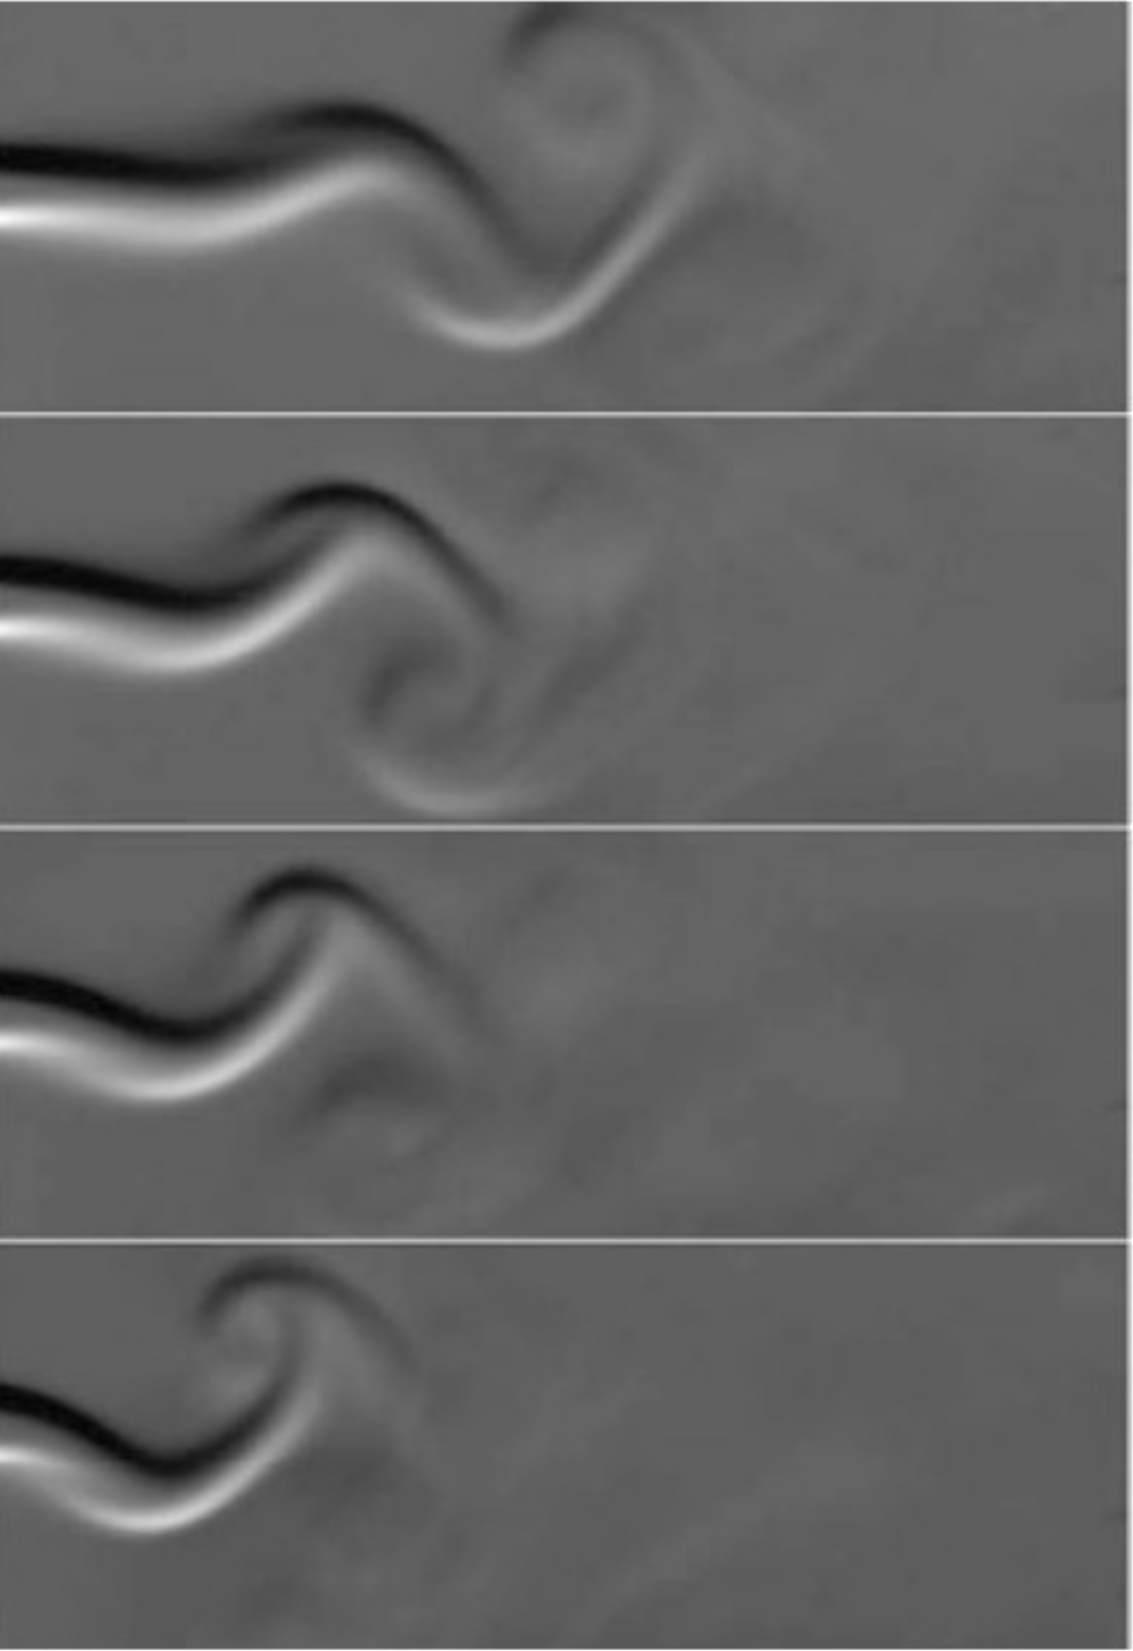
\includegraphics[height=0.3\textheight]{00_Images/07_chapter/14.png}
        \label{fig:jettransverse}
    } \hfill
    \subfloat[Turbulent Jet]{
        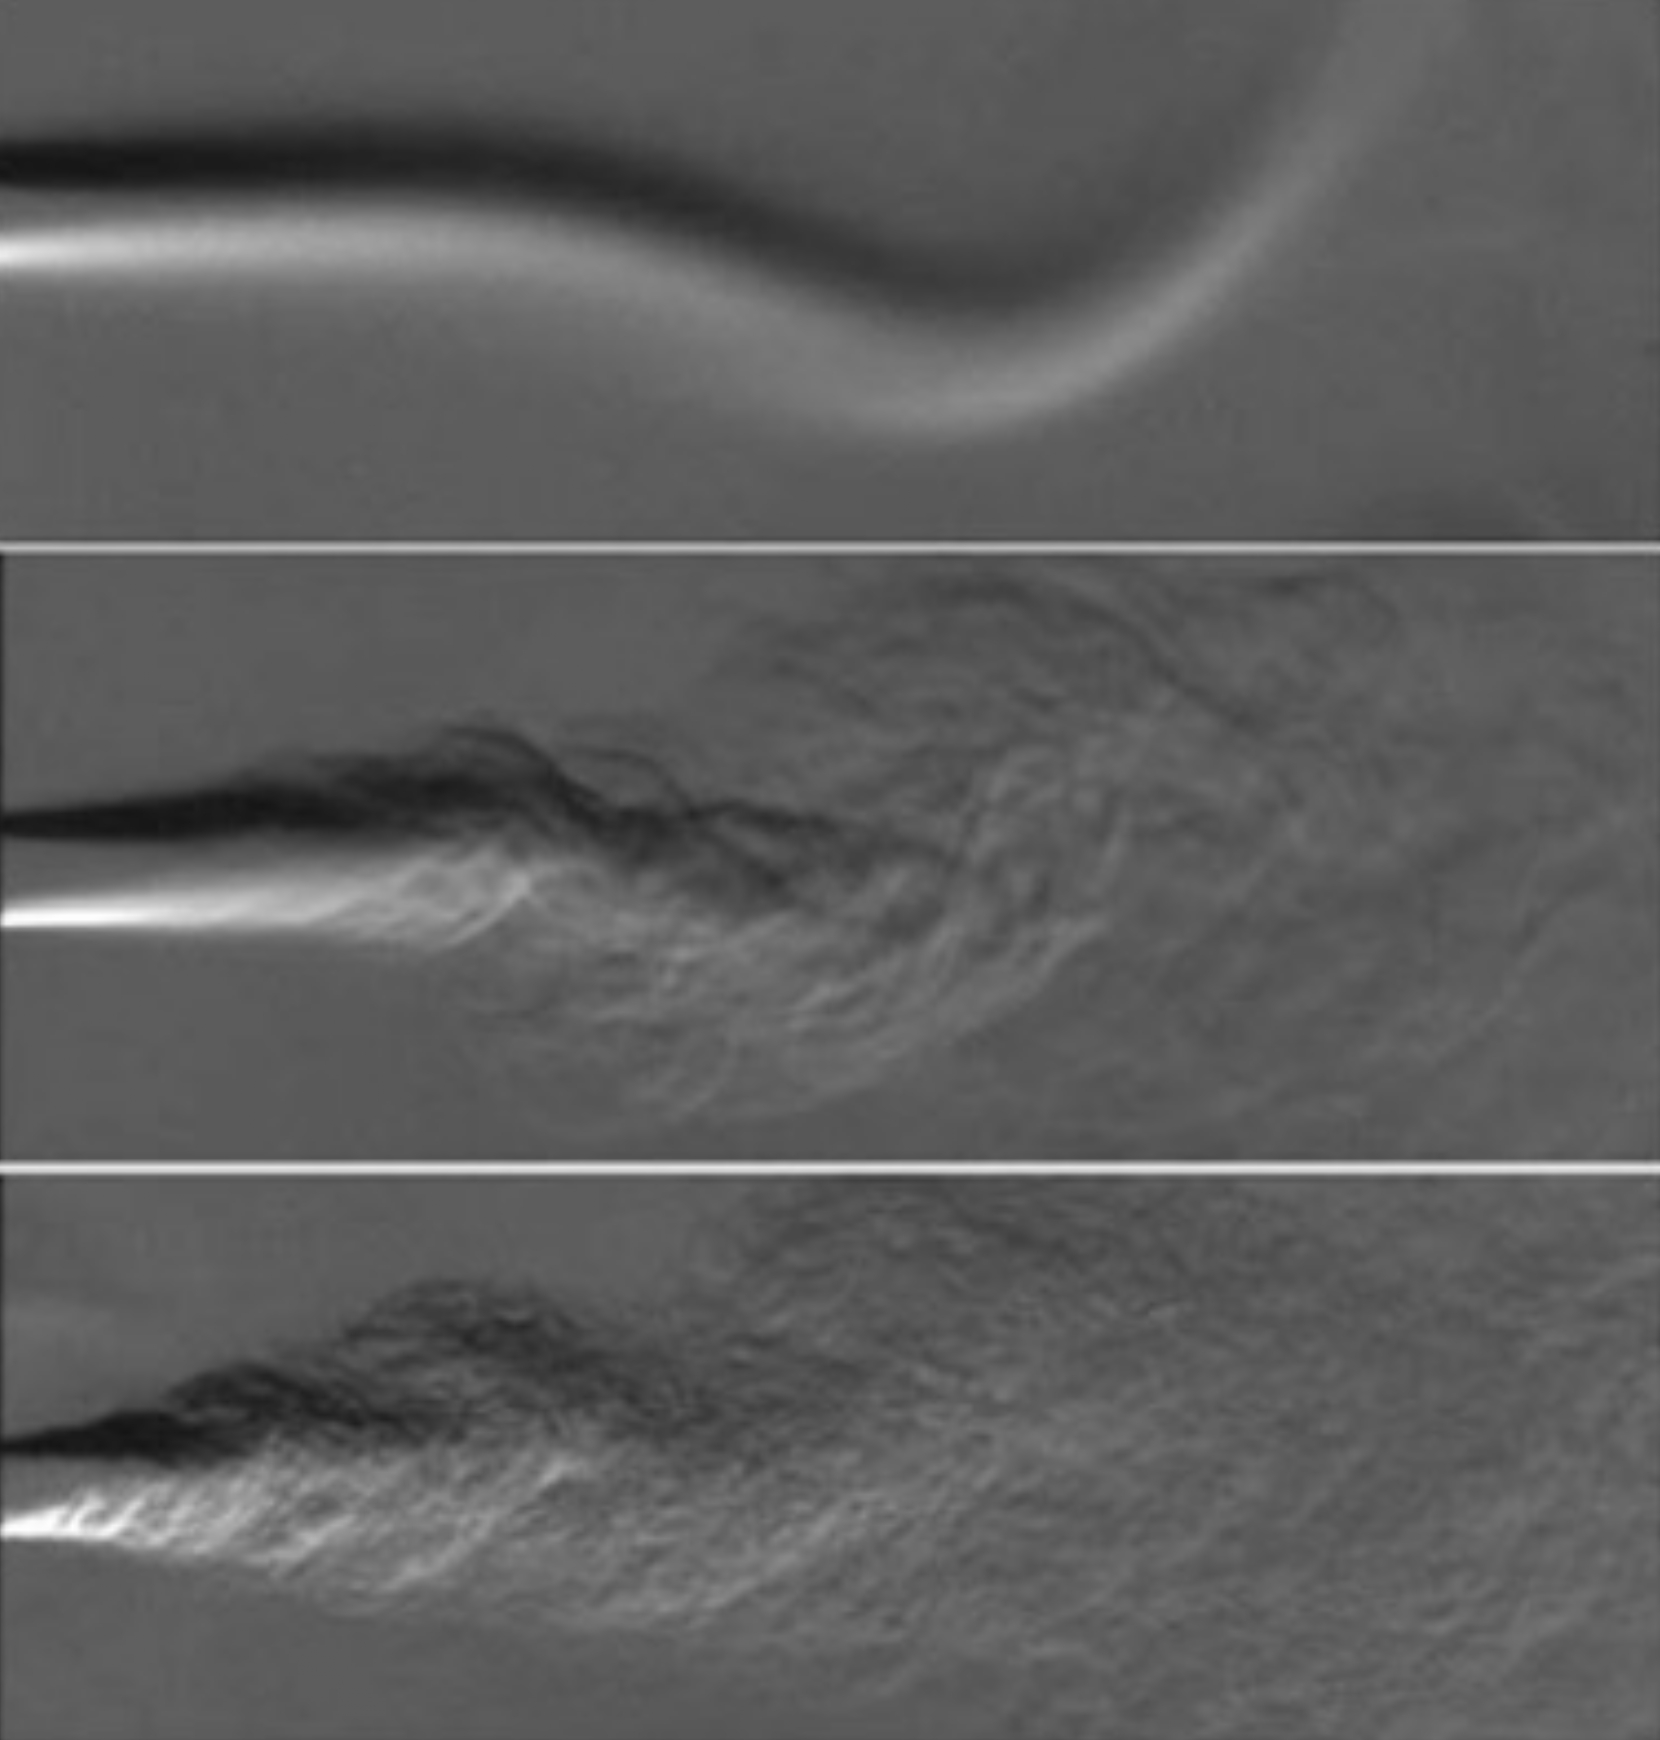
\includegraphics[height=0.3\textheight]{00_Images/07_chapter/15.png}
        \label{fig:turbolent}
    }
    \caption{Visualization of a jet subject to a transverse acoustic field and of a jet perturbed by an acoustic field}
\end{figure}

\section{The Aeroacoustic Source}

The interaction of the oscillating jet with the labium produces the acoustic energy that sustains the oscillation in the resonator. The largest jet oscillation takes place at a position where the resonator shows a strong reaction: the labium is an edge at an open pipe end, where the acoustic velocity is maximum. Furthermore, a sharp labium induces a local singularity in the acoustic field. The same jet oscillation in the free field or at a less reactive position in the resonator would not produce as much sound.

\section{The Jet-Drive Model}

\begin{figure}
    \centering
    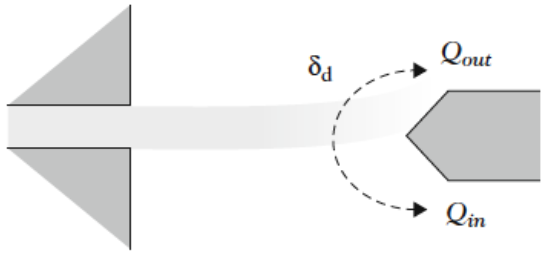
\includegraphics[width=0.7\linewidth]{00_Images/07_chapter/16.png}
    \caption{The jet-drive model}
    \label{fig:jetdrivemodel}
\end{figure}

\subsection{Dipole Source Representation}

This model is based on an idea by Helmholtz and Rayleigh. The model takes the two flow injections on both sides of the labium into account. The two sources (referencing to figure \ref{fig:jetdrivemodel}) \(Q_{\mathrm{in}}\) and \(Q_{\mathrm{out}}\) have fluctuating parts \(Q_1\) and \(Q_2\), placed a small distance \( \delta_d \) from each other, with opposite phases. They generate a pressure difference.

\subsection{Low-Frequency Approximation and Resonator as a Transmission Line}

The model is developed using a low-frequency approximation. Plane waves propagate in the resonator, which is therefore represented as a 1D transmission line. Assuming that the source dimensions are small compared to the acoustic wavelength, the resonator is described as the composition of a main pipe and a short, thinner pipe, since the open end in the mouthpiece always has a smaller cross-sectional area than the pipe.

\subsection{Force on the Acoustic Field}

The two sources with opposite phases \(Q_1\) and \(Q_2\) are placed in the thin short pipe at a short distance \( \delta_d \) from each other. They constitute a dipole confined in the small pipe of cross section \(S_m\) and produce an alternate motion of the air mass \( \rho\delta_d S_m \) between the two sources. The acceleration of this air mass generates the force acting on the acoustic field. This force can be expressed in terms of a pressure difference acting across the mouth of the pipe using the Euler equation.
\[
\frac{\partial p}{\partial x}=-\rho\frac{du}{dt} 
\quad \Rightarrow \quad
\frac{\Delta p}{\delta_d} \approx - \frac{\rho}{S_m} \frac{d Q_1}{dt}
\]

\subsection{Low Jet Velocity Relations}

For low jet velocities (Reynolds number below several hundred), it can be stated that
\[
\delta_d \approx \frac{\lambda_h}{2}
\qquad
\lambda_h=\frac{2\pi c_p}{\omega}
\qquad
c_p=\frac{\omega}{\alpha_r}
\]
In many cases,
\[
c_p=0.4U_j
\]
Defining \( \eta \) as the jet transverse displacement at the labium,
\[
Q_1 = H\int_{y_0}^{\infty}U(y-\eta)dy
\]
where \(H\) is the width of the jet at the labium. In many cases, \(H=h\) (flue channel thickness) and \(y_0\) is the transverse position of the labium. The displacement at the labium can be written as
\[
\eta(W,t)=\frac{h}{U_j}v_{\mathrm{ac}}\left(t-\frac{W}{c_p}\right)e^{\alpha_i W}
\]

\subsection{High Jet Velocity Scaling}

For high jet velocities, the acoustic power varies as the fourth power of the jet velocity, i.e., the Mach number,
\[
P_{\mathrm{ac}}\propto M^{4}
\qquad
M=\frac{U_0}{c}
\]
In sound synthesis by physical modeling, adding a broadband noise that follows this power law to the source terms improves the realism of the synthesis.

\subsection{Flow-Driven Excitation}

Since the deflection of the jet is the acoustic driving mechanism and since this is driven by the acoustic flow out of the mouth of the resonator, the system will work best when this flow is a maximum and therefore at an acoustic admittance maximum. This corresponds to a flow-driven excitation mechanism. This is in contrast with pressure-driven reed generators, which operate at an impedance maximum of the resonator.

\section{Nonlinearity and Harmonic Generation}

\subsection{Jet Velocity Profile}

Let us analyze what happens when there is an offset between the labium position and the flue channel exit. The velocity profile of the jet tends toward a smooth, bell-shaped form described by
\[
U(y) = U_0 \sech^{2}\left(\frac{y}{b}\right)
\]
where \(U_0\) and \(b\) vary along the jet.

\subsection{Flow into the Resonator with Labium Offset}

Consider the flow into the resonator when the jet tip is displaced by an amount \(h\) and the labium is displaced by \(h_0\) from the center of the jet. The corresponding flow is
\[
U_j
= W\int_{-\infty}^{h_0} U_0 \sech^{2}\left(\frac{y-h}{b}\right)dy
= W b U_0\left[\tanh\left(\frac{h_0-h}{b}\right) + 1\right]
\]
A jet with a top-hat velocity profile would yield a similar characteristic but with a sharper change in slope. This behavior is reported in figure \ref{fig:resonatorflow}.

\begin{figure}[!htb]
    \centering
    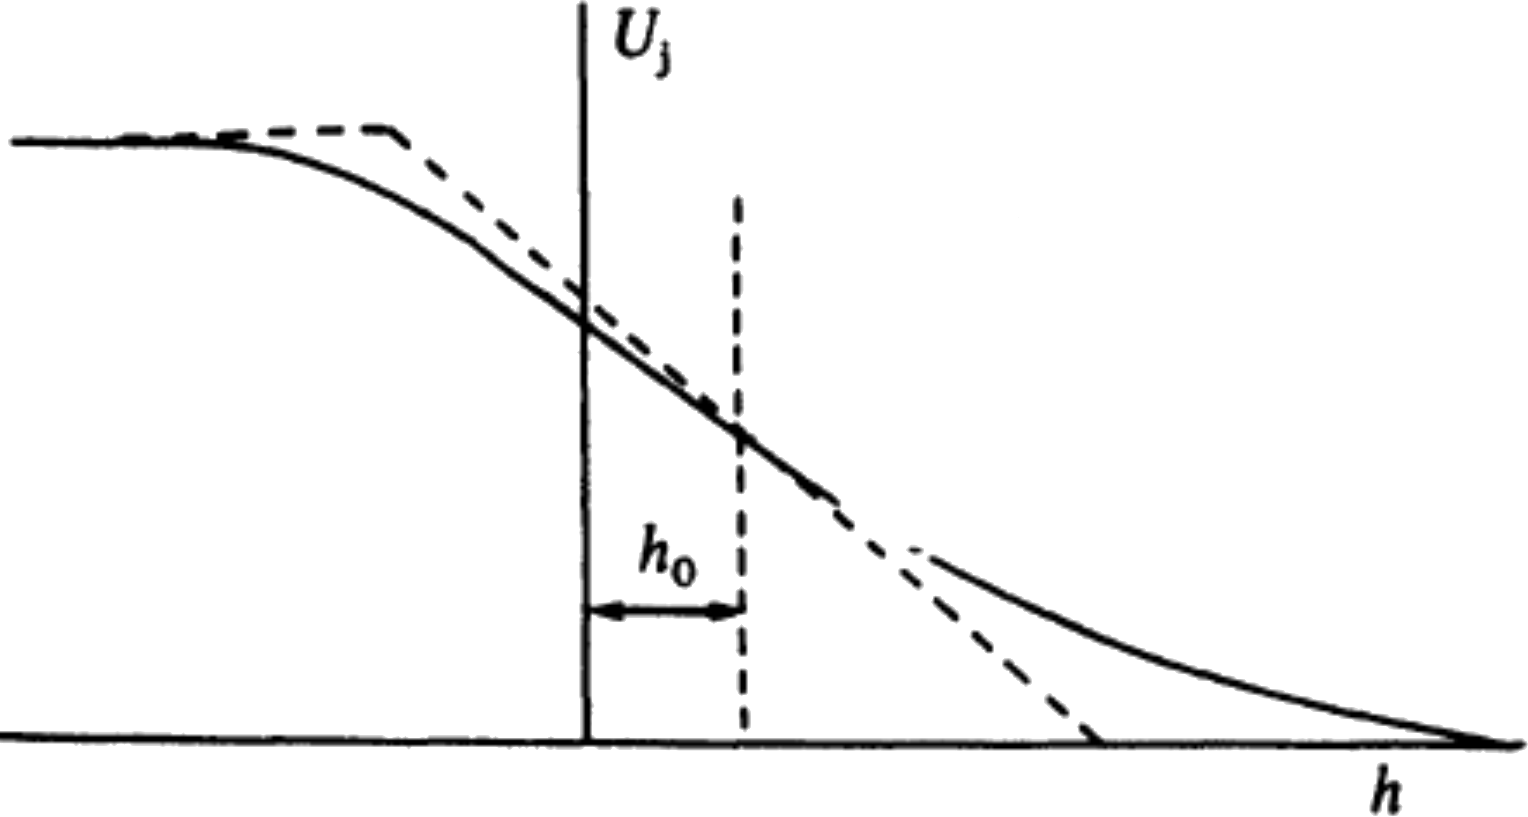
\includegraphics[width=0.7\linewidth]{00_Images/07_chapter/18.png}
    \caption{The flow into the resonator with labium offset}
    \label{fig:resonatorflow}
\end{figure}

\subsection{Sinusoidal Excitation and Harmonics}

Assume that the excitation is sinusoidal,
\[
h = a\cos\omega t
\]
If \(a<b\), the amplitude of the \(n\)-th harmonic varies approximately as \((a/b)^n\) and there is also a dependence on \(h_0/b\). If \(h_0=0\) the jet strikes the labium symmetrically and there are no even harmonics. If \(h_0 = 1.1b\), there is no third harmonic, but the first and second are strong. As an example, relative levels of the first four harmonics of the jet drive of an organ pipe as a function of the ratio of the offset \( h_0 \) of the jet relative to the jet half-width b are reported in figure \ref{fig:organflow}.

\begin{figure}[!htb]
    \centering
    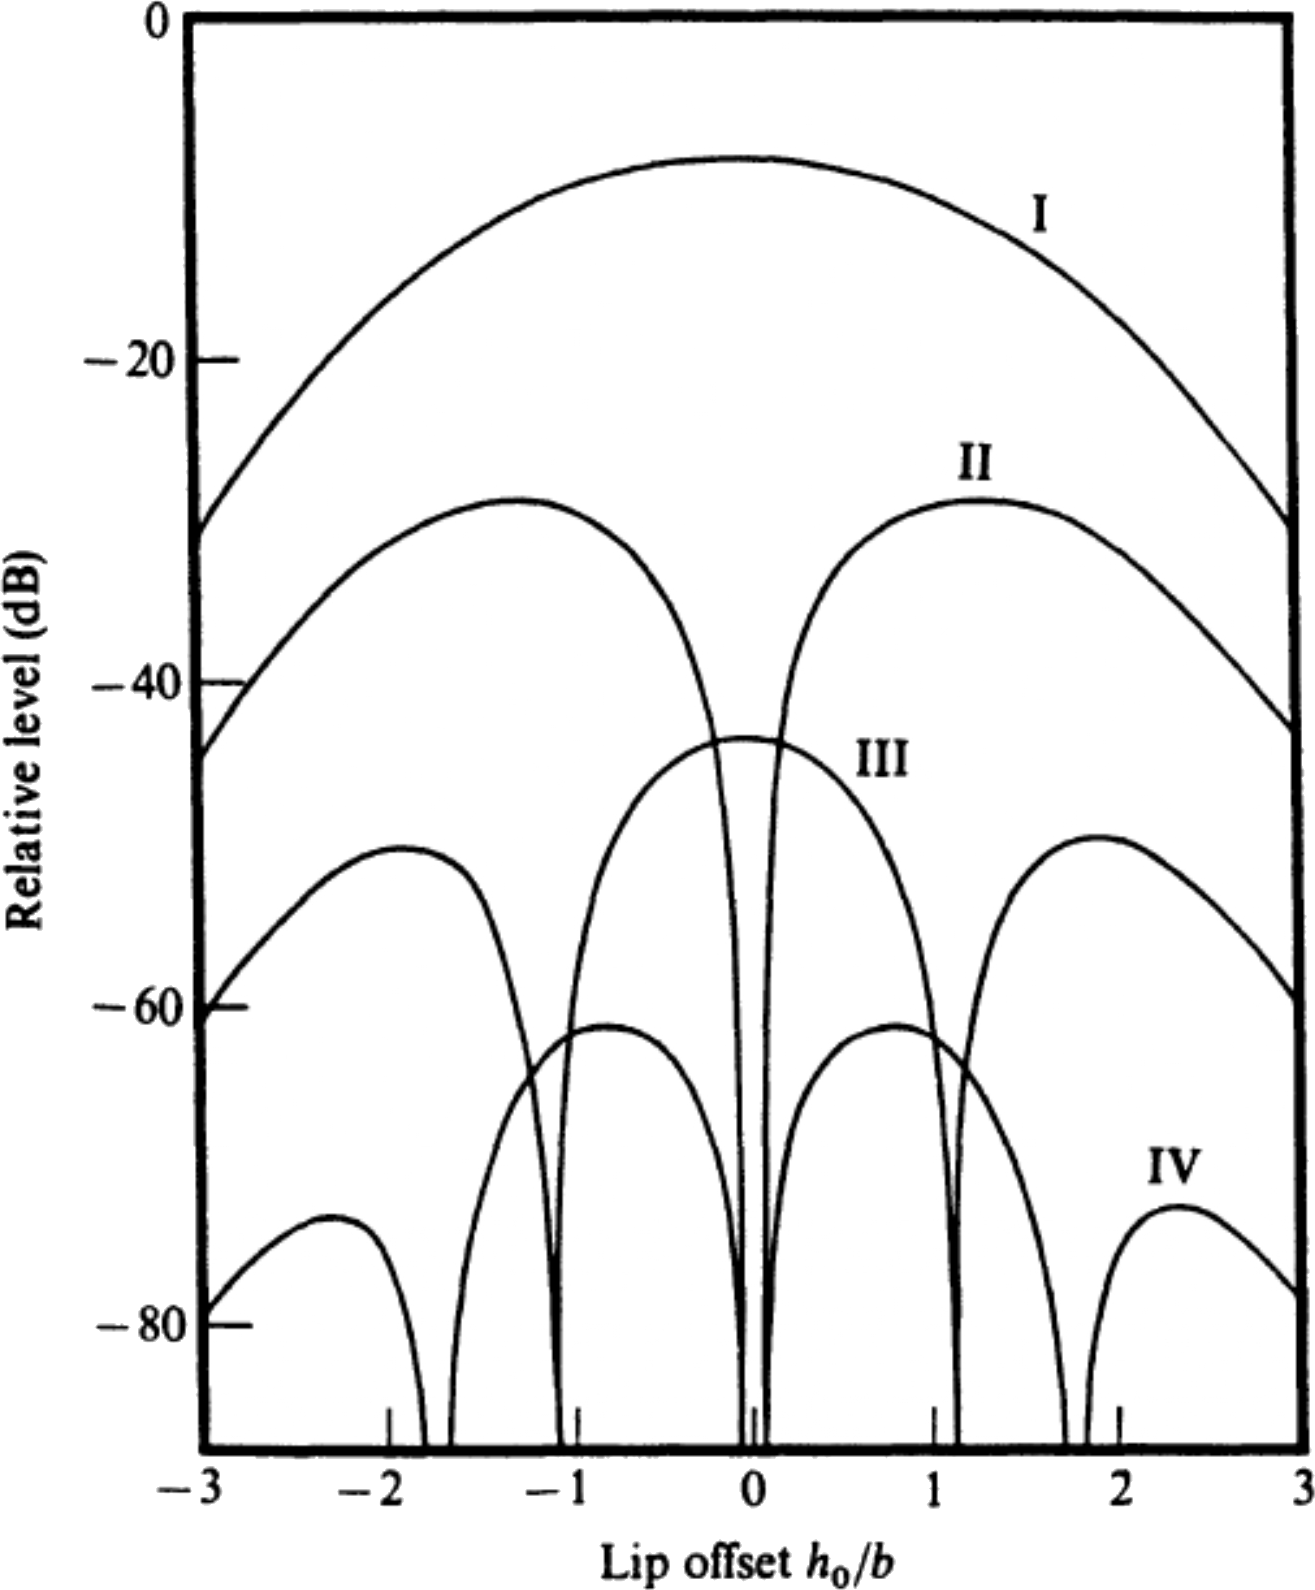
\includegraphics[height=0.3\textheight]{00_Images/07_chapter/19.png}
    \caption{Levels of the first four harmonics of the jet drive of an organ pipe}
    \label{fig:organflow}
\end{figure}

\subsection{Interaction With Pipe Resonances}

The presence of any upper harmonics in the pipe flow will be reflected in propagating waves of appropriate frequency on the jet and, consequently, in the further drive terms. The effect of this interaction is relatively small unless the jet length and velocity are such that it acts as a generator at the harmonic frequency. The relative level of upper harmonics in the sound is greatly influenced by the frequency alignment and \(Q\)-values of the upper pipe resonances.

\section{An Overview on Flute-Type Instruments}

\subsection{Panpipes and Shakuhachi}

The simplest type of flute-like instrument is the panpipes. There is a single pipe resonator for each note, made from bamboo cut so that its lower end is closed by a septum in the plant stem. The adjustment of the pipe length is then accomplished by pouring wax into the pipes. The instrument generally produces a simple diatonic major scale over a compass of about 1.5 to 2 octaves and is sounded by blowing across the top of each pipe, with the player's lower lip in contact with one edge of the pipe opening. The pipes are scaled so that their cross-sectional area is roughly proportional to length: long pipes are relatively narrower than short pipes. An incidental effect of the scaling of pipe diameter is a consequent scaling of jet length, which aids in the sounding of high notes. Since the jet length is decreased by a factor \(1/\sqrt{2}\) for an octave change in pitch, it is necessary to increase the jet speed by a factor \(\sqrt{2}\) or the blowing pressure by a factor \(2\) to maintain the appropriate phase relations. Since the pipe resonators are stopped at their lower ends, their resonance frequencies follow approximately an odd-harmonic series. Percussive breathy sounds can also be produced by deliberately failing to satisfy the normal regeneration conditions and blowing with a wide, turbulent jet; the acoustic spectrum then resembles the noise background. The shakuhachi is made from the root end of a bamboo plant and constitutes a nearly cylindrical, slightly curved, open tube. The mouth end has a bevel cut on one side that is fashioned to a sharp edge or may even have an ivory or agate wedge inserted. The player blows across the open end, but more into the instrument than for the panpipes. Since the tube is open, odd and even harmonics are comparably strong in the radiated sound. The shakuhachi has just five finger holes (two for the fingers of each hand and one for the left thumb) and is naturally adapted for traditional Japanese pentatonic music.

\subsection{The Recorder}

In the recorder family, the air jet is defined by an extended slit or windway; the shape of the mouth and labium is defined by the construction of the instrument and the notes of the scale are produced by opening finger holes. With the exception of the ocarina, the instruments of this family use a cylindrical or slightly tapering air column rather than a flaring one. Recorders have a very long history, but they are commonly divided into Renaissance recorders and Baroque recorders. Renaissance recorders have a nearly cylindrical bore and a simple outside form, while instruments of the Baroque style have a tapering conical bore, two or more separately jointed sections and decorative turning near the head and foot. Baroque recorders are made in a wide range of sizes.

\subsection{Recorder Bore and Resonance Conditions}

Neglecting the radiation load, an incomplete cone can be characterized through its input impedance \(Z_{\mathrm{in}}\), leading to the usual distinction between impedance zeros and impedance maxima. In particular, impedance maxima occur when \(\sin k(L+\theta_1)\) vanishes and relative to a cylindrical bore, the maxima are raised in frequency and do not lie midway between minima. The most relevant advantage of the conical bore with respect to the cylindrical one is constructional: careful tuning requires adjustments of the bore diameter at various places along its length, which can be built into a tapered reamer with consequent ease of adjustment and reproducibility. In a typical Baroque recorder, the main-bore taper corresponds to a conical semi-angle between \(0.5^\circ\) and \(1^\circ\) and the diameter at the foot end is typically \(0.5\) to \(0.7\) times that at the head. The resonance condition for the whole instrument is that the impedance of the air column in series with the impedance of the mouth window be a minimum. The mouth impedance \(Z_m\) is essentially an inertance \(j\omega M\). Equating the low-frequency form of a cylindrical-bore end correction to this inertance yields the constraint
\[
\Delta L = \frac{MS}{\rho}
\]
However, \(\Delta L\) decreases with frequency. This tends to stretch the intonation: high-note resonances are sharp and low-note resonances are flat. Players compensate by blowing low notes as strongly as possible to raise pitch and doing the opposite for high notes.

\subsection{The Flute}

With the term flute we refer typically to the transverse flute. Before Baroque times, flutes were generally cylindrical and this form was revised in the late seventeenth century. The Baroque flute, like the recorder, had a slightly tapered conical main bore and was divided into two or more sections, the head being nearly cylindrical. It had six main finger holes, an extra hole for the right-hand little finger and no thumb hole. Unlike the recorder, the flute continued to develop and progressively acquired keys between and below the six normal finger holes to allow accurate and even playing of chromatic semitones. The modern flute has a cylindrical bore about \SI{19}{\milli\meter} in diameter, except for the head joint, which contracts slightly to about \SI{17}{\milli\meter} toward the embouchure hole. It has 12 or 13 large holes and 3 small ones, all covered by padded keys and a unified mechanism that allows virtually any combination of holes to be closed without moving the fingers from their standard positions.

\subsection{Flute Head Joint: Cavity and Embouchure Hole}

\begin{figure}[!htb]
    \centering
    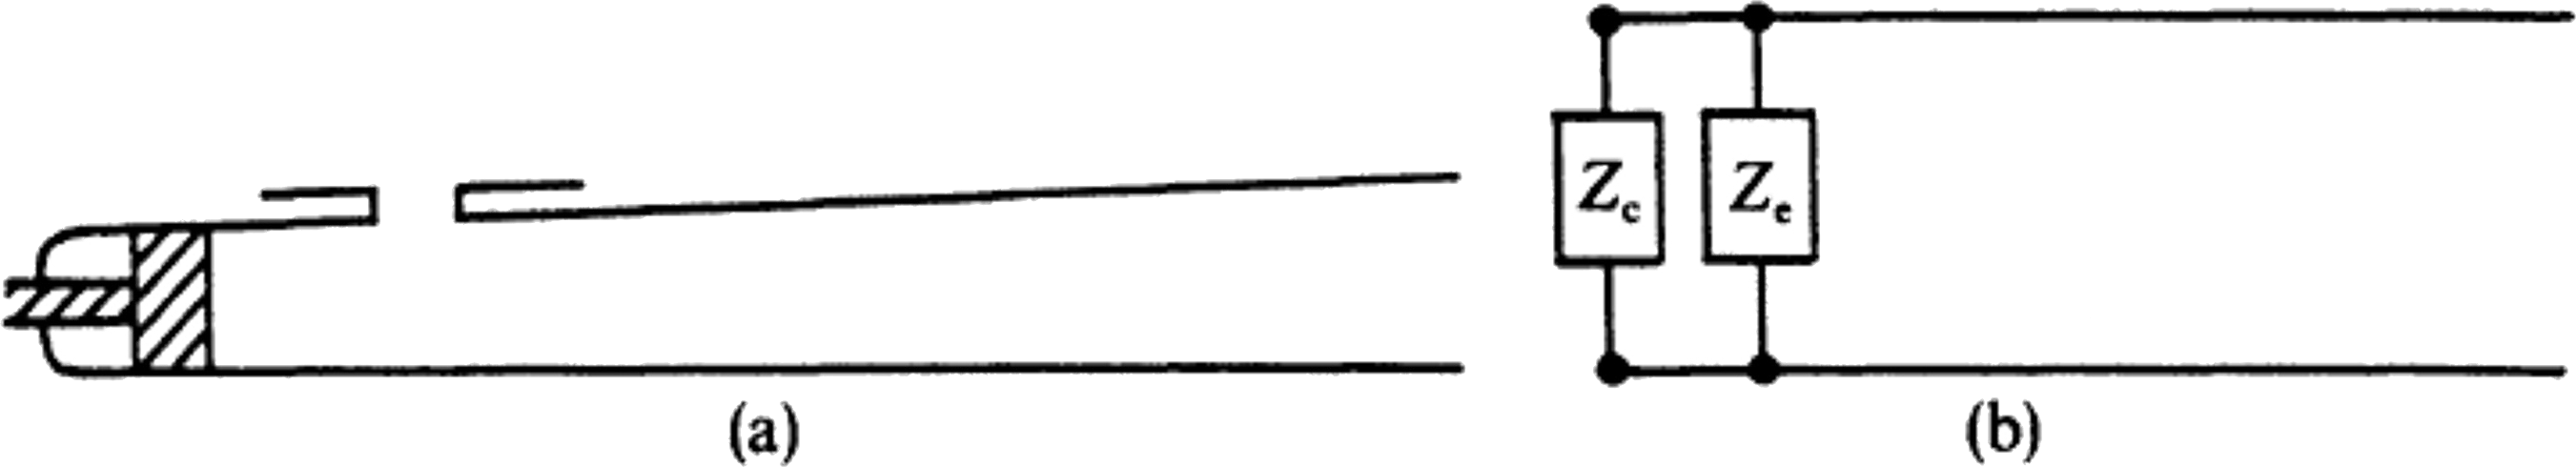
\includegraphics[width=0.7\linewidth]{00_Images/07_chapter/20.png}
    \caption{Tapered head joint of a modern flute and its equivalent network}
    \label{fig:flutescheme}
\end{figure}

Most important to the tuning and tonal quality of a flute are the bore profile of the head joint, the size of the cavity between the embouchure hole and the stopped end and the detailed shape of the embouchure hole. Of these, the most significant is the cavity above the embouchure hole: gross mispositioning of the stopper cork defining this cavity can mistune the two lower registers by as much as half a semitone relative to each other. Considering the scheme reported in figure \ref{fig:flutescheme}, the embouchure impedance \(Z_e\) is that of an inertance \(M\),
\[
Z_e = jM\omega = j\frac{\rho l_e \omega}{S_e}
\]
and the shading effect of the player’s lips must be taken into account in evaluating \(l_e\) and \(S_e\). The cavity impedance \(Z_c\) is that of an acoustic compliance \(C\),
\[
Z_c = \frac{1}{j\omega C} = -j\frac{\rho c^2}{\omega V}
\]
The characteristic impedance of the flute tube is
\[
Z_0 = \frac{\rho c}{S}
\]
and the impedance presented by embouchure hole and cavity in combination is equivalent to an end correction \(\Delta L\) defined by
\[
jZ_0\tan k\Delta L = (Z_e^{-1} + Z_c^{-1})^{-1}
\]
or
\[
\Delta L
= \frac{c}{\omega}\tan^{-1}\left[\frac{M\omega}{Z_0\bigl(1-MC\omega^2\bigr)}\right]
\]
In a normal head joint, \(\Delta L\) can be made nearly constant over the range \(0\)–\SI{2}{\kilo\hertz} if the stopper is set about \SI{17}{\milli\meter} from the center of the embouchure hole and \(\Delta L\) is then about \SI{42}{\milli\meter} with the player’s lips in normal position. Another important component is the embouchure hole itself. Early wooden flutes had a wall thickness at the head joint of about \SI{5}{\milli\meter} and almost any hole of reasonable size (e.g. \SIrange{7}{12}{\milli\meter} diameter) could function as an embouchure hole. For an average player, a hole about \SI{10}{\milli\meter} in diameter is best: a smaller one gives a soft, constricted sound, while a larger one is loud but less controlled. Boehm introduced a nearly rectangular hole, with dimensions close to \SI{10}{\milli\meter} by \SI{12}{\milli\meter}. In a metal flute the hole is built up using a chimney about \SI{5}{\milli\meter} in height, on top of which is the embouchure plate against which the player's lower lip rests.
